%!TEX program = xelatex

% Name           : hsrm-beamer-demo.sty
% Author         : Benjamin Weiss (benjamin.weiss@kreatiefton.de)
% Version        : 0.4
% Created on     : 05.05.2013
% Last Edited on : 24.03.2014
% Copyright      : Copyright (c) 2013-2014 by Benjamin Weiss. All rights reserved.
% License        : This file may be distributed and/or modified under the
%                  GNU Public License.
% Description    : HSRM beamer theme demonstration. Also includes a short 
%                  Tutorial regarding the beamer class.

\documentclass[compress, noflama]{beamer}
%--------------------------------------------------------------------------
% Common packages
%--------------------------------------------------------------------------
\usepackage[french]{babel}
\usepackage{multimedia}
%\usepackage{movie15}
\usepackage{graphicx}
\usepackage{multicol}
\usepackage[scale=2]{ccicons}
% Erweiterte Tabellenfunktionen
%\usepackage{tabularx,ragged2e}
\usepackage{booktabs}
\usepackage{appendixnumberbeamer}
% Listingserweiterung
%\usepackage{listings}
%\lstset{ %
%language=[LaTeX]TeX,
%basicstyle=\normalsize\ttfamily,
%keywordstyle=,
%numbers=left,
%numberstyle=\tiny\ttfamily,
%stepnumber=1,
%showspaces=false,
%showstringspaces=false,
%showtabs=false,
%breaklines=true,
%frame=tb,
%framerule=0.5pt,
%tabsize=4,
%framexleftmargin=0.5em,
%framexrightmargin=0.5em,&
%xleftmargin=0.5em,
%xrightmargin=0.5em
%}

%--------------------------------------------------------------------------
% Load theme
%--------------------------------------------------------------------------
\usetheme{metropolis}

%\usepackage{dtklogos} % must be loaded after theme
%\usepackage{tikz}
%\usetikzlibrary{mindmap,backgrounds}
%--------------------------------------------------------------------------
% General presentation settings
%--------------------------------------------------------------------------
\title{Introduction à l'haptique et à la perception du mouvement}
\subtitle{Cours Master}
\date{15 Novembre 2022}%Mise à jour: \today}
\author{Fabien Danieau}
\institute{Pollen Robotics\\ \href{mailto:fabien.danieau@interdigital.com}{fabien.danieau@pollen-robotics.com}}
\titlegraphic{\hfill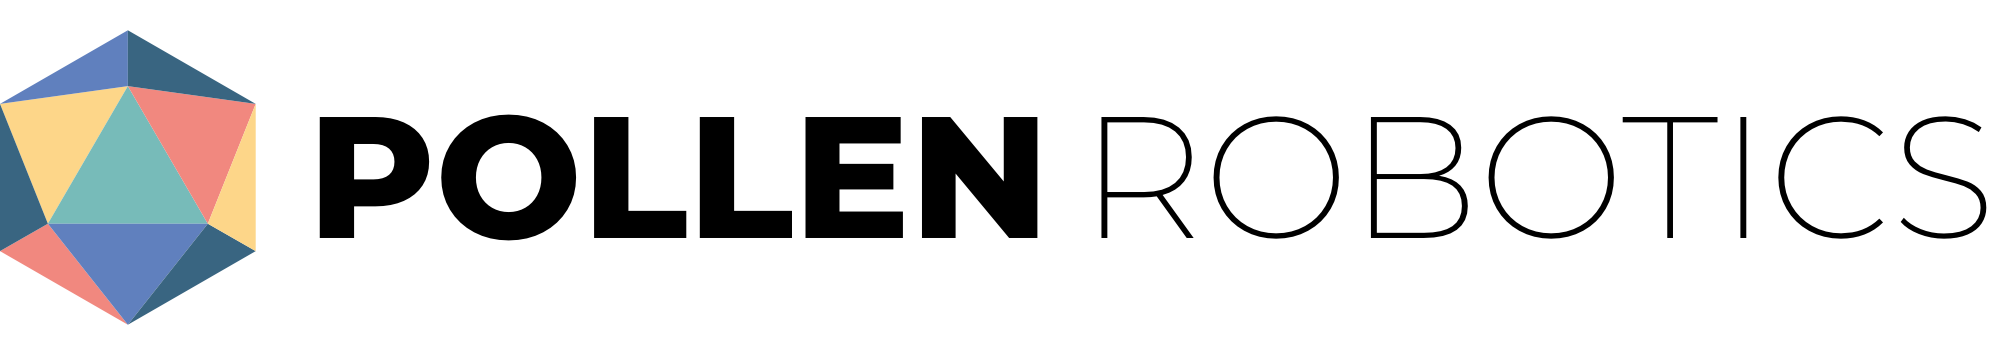
\includegraphics[width=5cm]{new_logo_pollen_rectangle.png}}
%--------------------------------------------------------------------------
% Notes settings
%--------------------------------------------------------------------------
%\setbeameroption{show notes}

\begin{document}
%--------------------------------------------------------------------------
% Titlepage
%--------------------------------------------------------------------------

\maketitle

%\begin{frame}[plain]
%	\titlepage
%\end{frame}

%--------------------------------------------------------------------------
% Table of contents
%--------------------------------------------------------------------------
\section*{Sommaire}
\begin{frame}{Sommaire}
	\setbeamertemplate{section in toc}[sections numbered]
	\tableofcontents[hideallsubsections]
\end{frame}

%--------------------------------------------------------------------------
% Content
%--------------------------------------------------------------------------
\setbeamercolor{hsrmSec1Demo}{fg=hsrmSec1,bg=white}

\section{Le sens Haptique}
\subsection{Définition}
{
\setbeamertemplate{frame footer}{\cite{johansson1987}}
\begin{frame}{Définition}
	\begin{itemize}
		\item Science du toucher
		\item Vient du grec \textit{haptesthai}: attraper, toucher
		\item Englobe les phénomènes \textcolor{teal}{tactiles} et \textcolor{blue}{kinesthésiques}%: perception du corps dans l'environement
	\end{itemize}
	
\begin{multicols}{3}

\begin{itemize}
\item \textcolor{teal}{Tactile}
\begin{itemize}
\setlength{\itemindent}{-0.5em}
\item \textcolor{teal}{Texture}
\item \textcolor{teal}{Vibration}
\item \textcolor{teal}{Force de friction}
\item \textcolor{teal}{Température}
\end{itemize}
\end{itemize}

\begin{figure}
		\centering			
		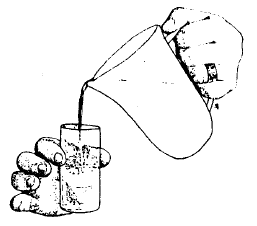
\includegraphics[width=\linewidth]{images/haptic}
		%\caption{\cite{johansson1987}}
	\end{figure}

\begin{itemize}
\item \textcolor{blue}{Kinesthésie}
\begin{itemize}
\setlength\itemsep{-0.2em}
\item \textcolor{blue}{Position}
\item \textcolor{blue}{Mouvement}
\item \textcolor{blue}{Force}
\item \textcolor{blue}{Résistance}
\end{itemize}
\end{itemize}

\end{multicols}	
	
\end{frame}
}

{
\setbeamertemplate{frame footer}{\cite{klatzky1990}}
\begin{frame}{Exploration haptique}
\begin{figure}
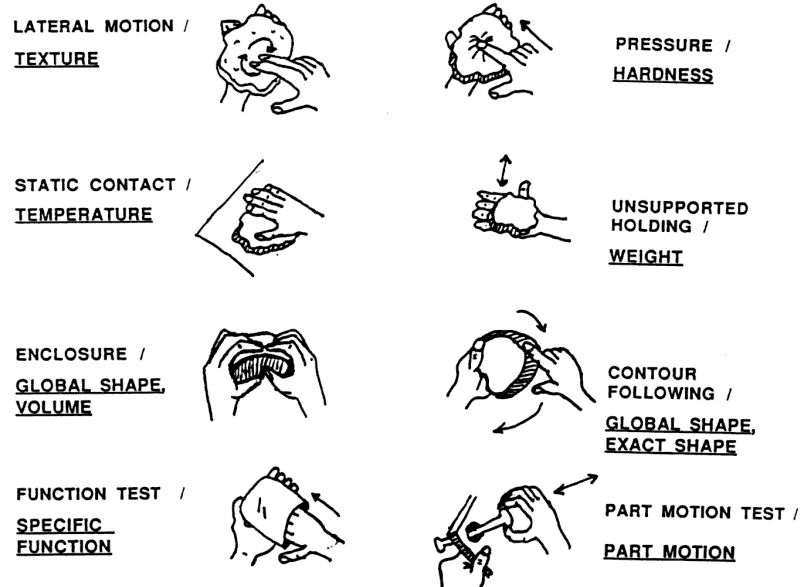
\includegraphics[width=9.5cm]{images/hapticExploration}
\end{figure}
\end{frame}
}

\subsection{Applications}
\begin{frame}{Exemples d'applications}
\begin{multicols}{2}
\begin{figure}
	\centering			
	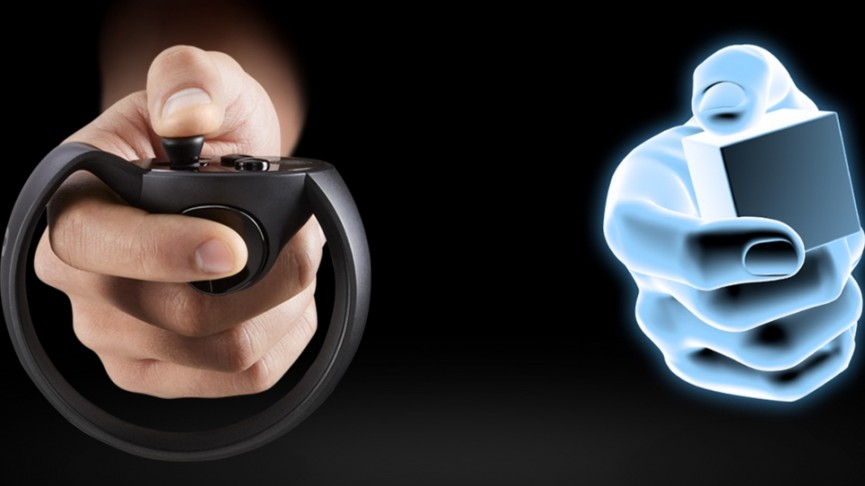
\includegraphics[width=4cm,height=2.7cm]{images/touch_vr}%{\copyright Nintendo}
	%\vspace{-0.5cm}
	\caption{Divertissement}
	\end{figure}
		\vspace{-0.7cm}	
	\begin{figure}	
	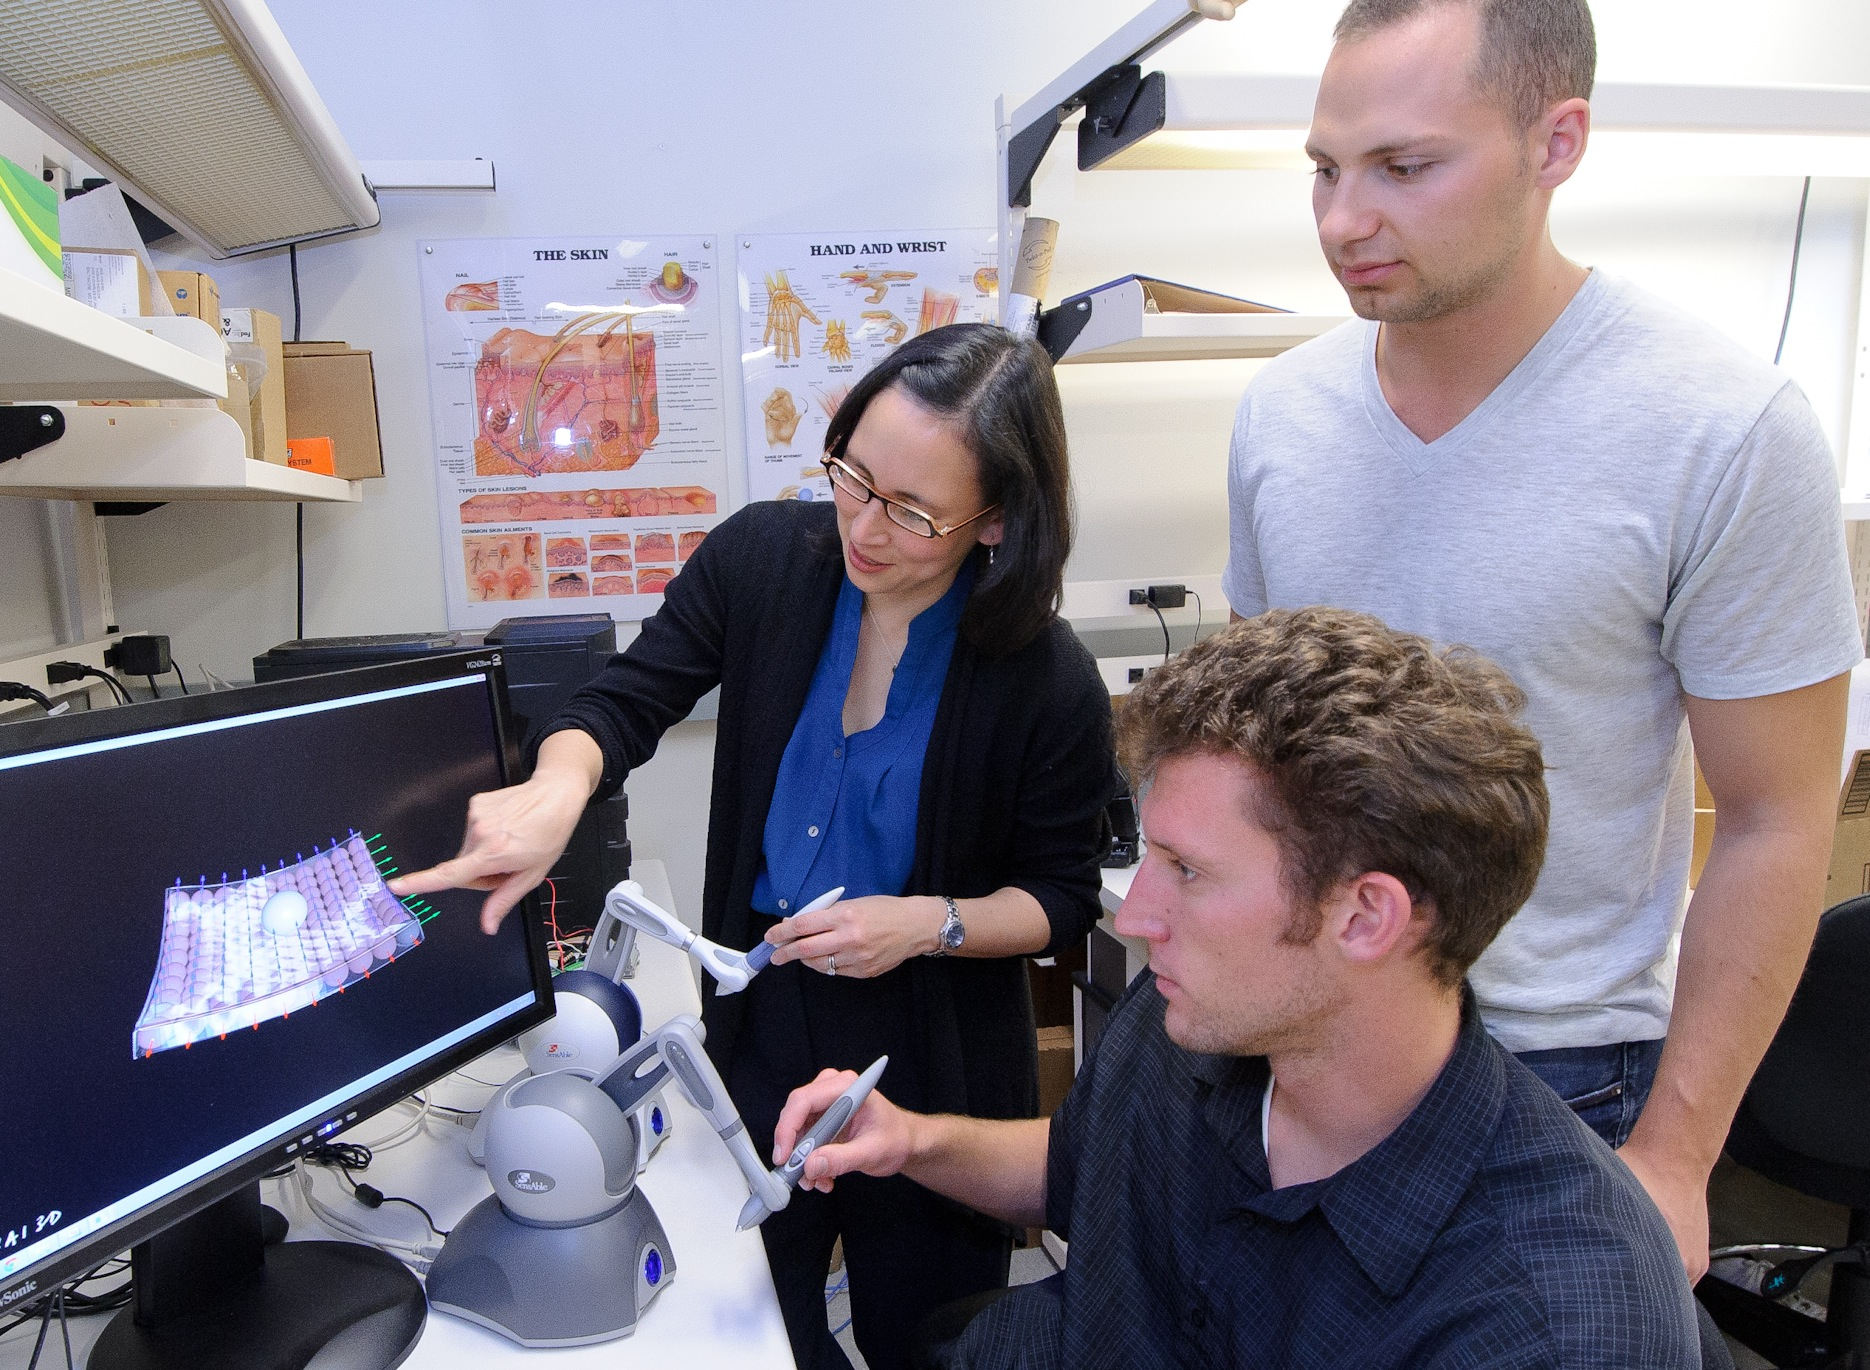
\includegraphics[width=4cm, height=2.7cm]{images/education}%{\copyright Stanford Charm Lab}
	%	\vspace{-0.5cm}
	\caption{Education}
	\end{figure}

\begin{figure}
	\centering			
	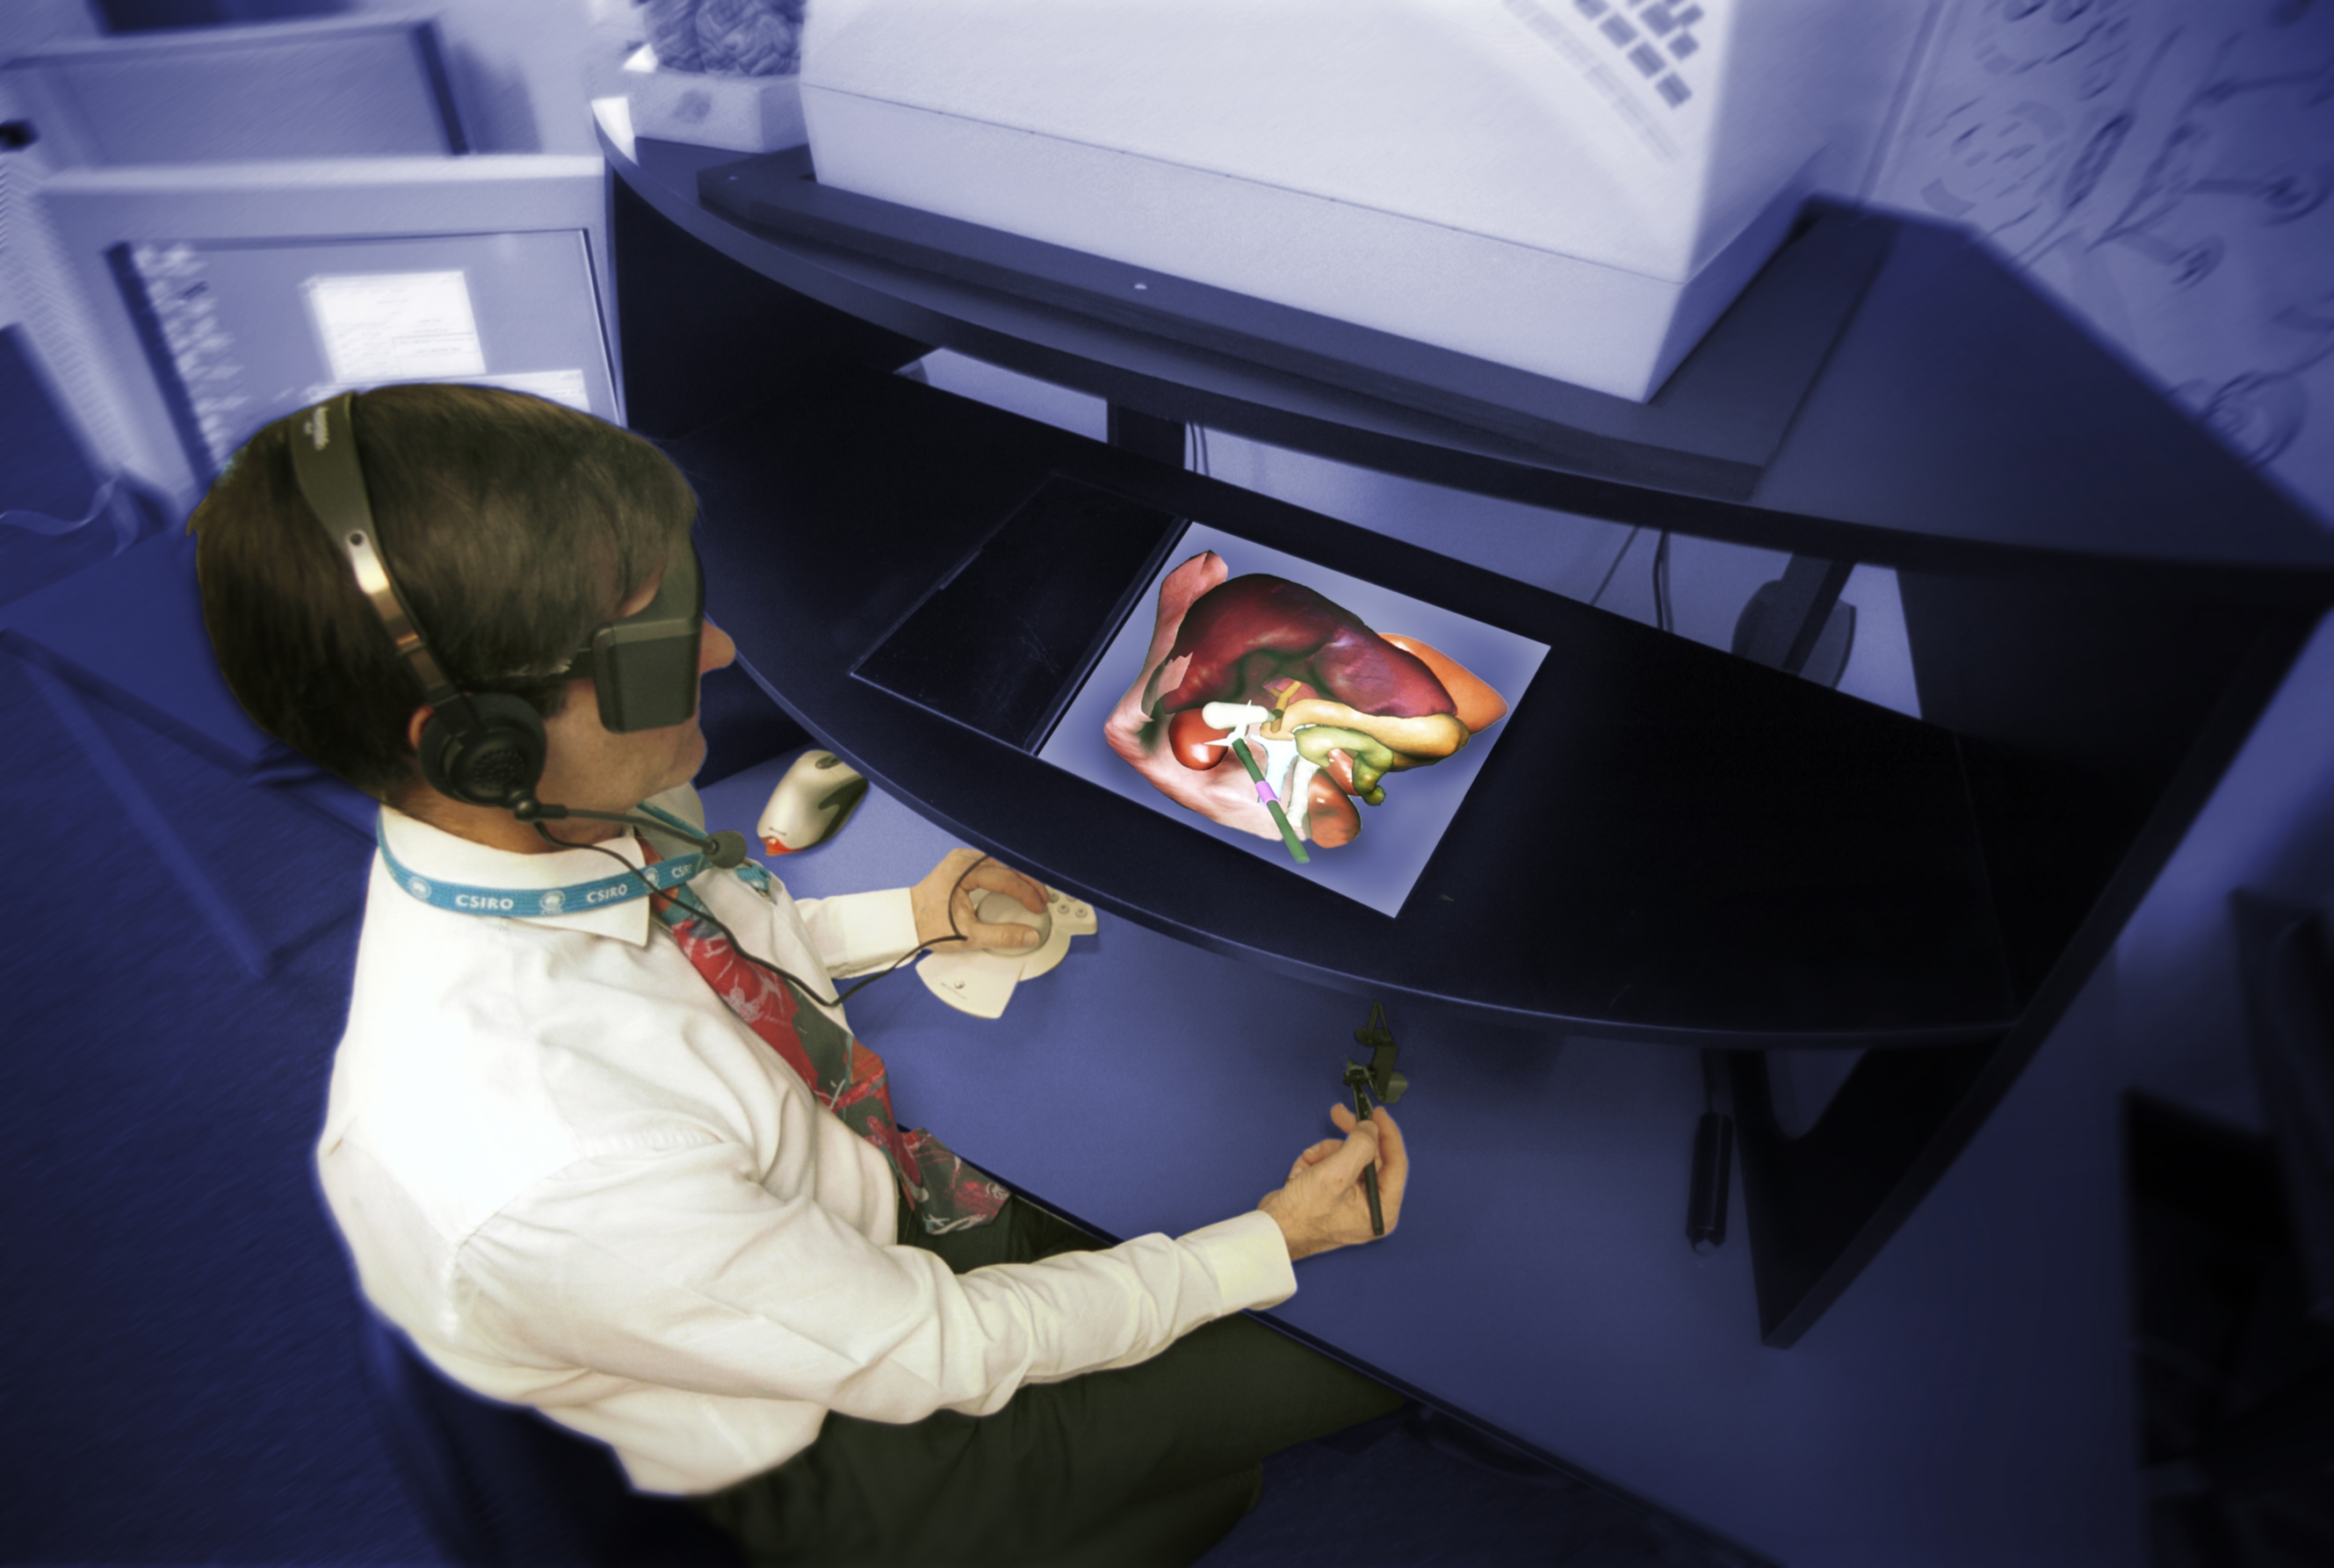
\includegraphics[width=4cm,height=2.7cm]{images/hapticSurgery}%{\copyright CSIRO}
	%	\vspace{-0.5cm}
	\caption{Médical}
		\end{figure}	
					\vspace{-1.5cm}	
	\begin{figure}
	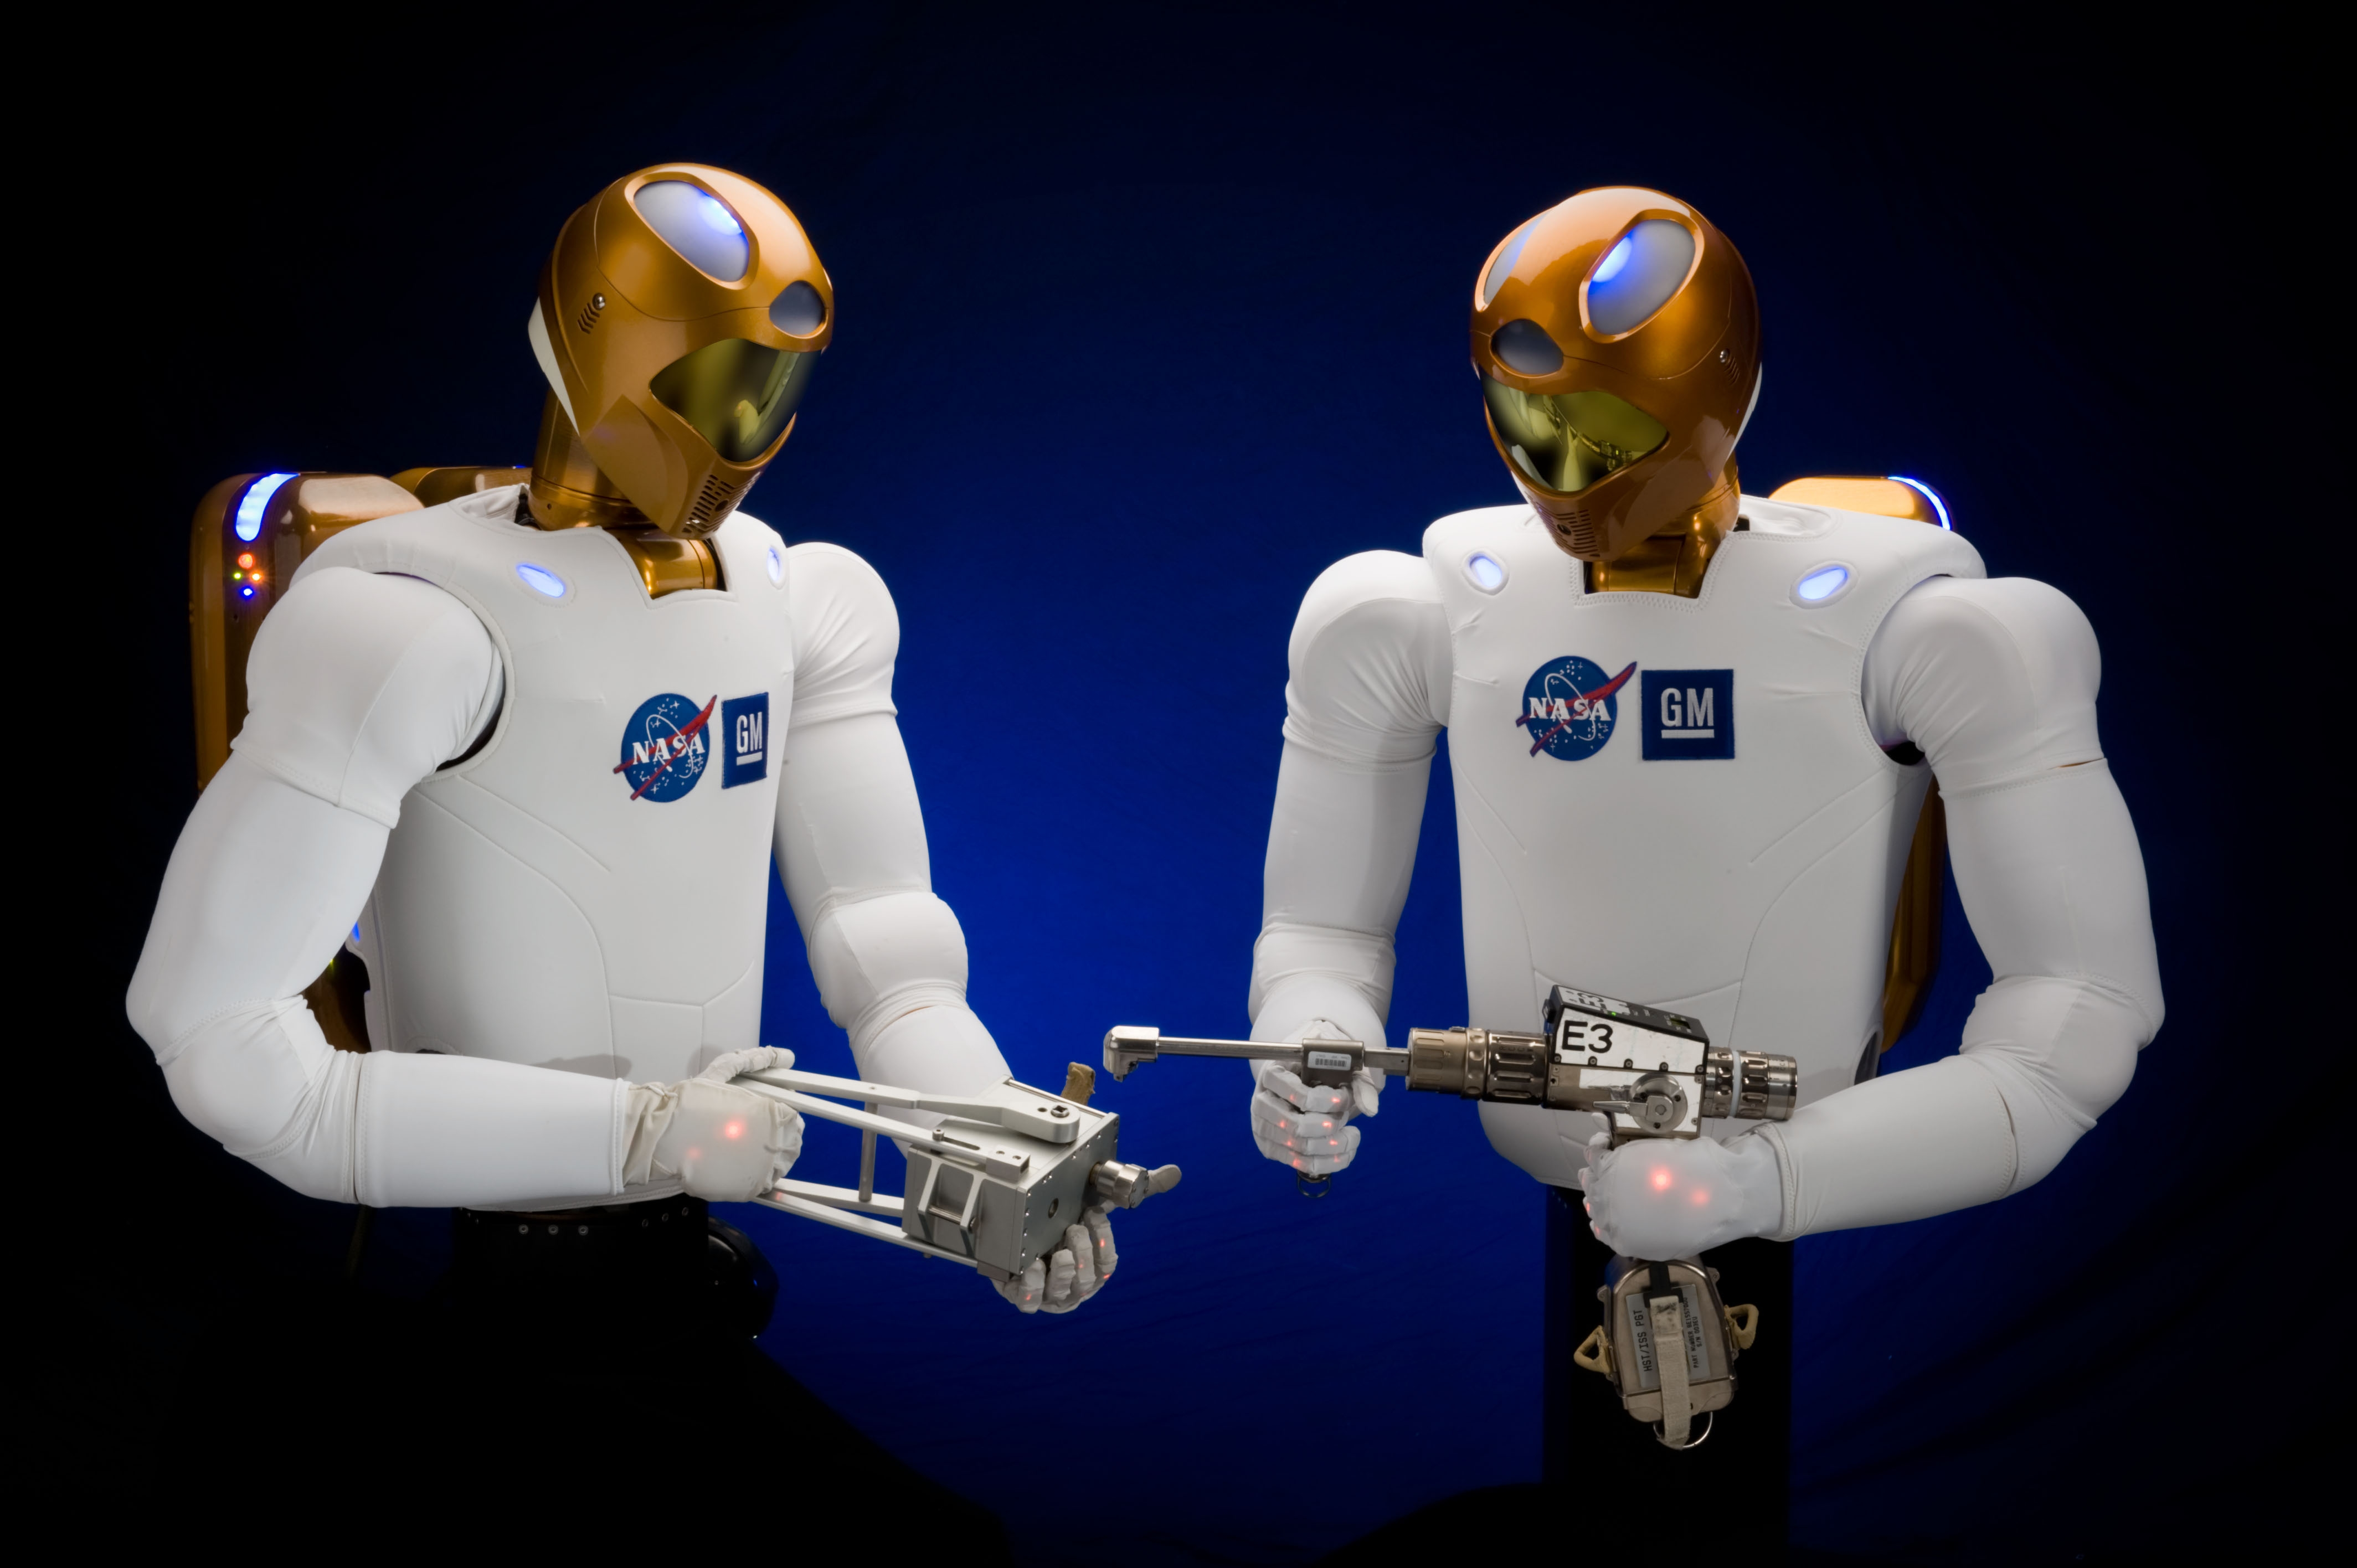
\includegraphics[width=4cm,height=2.7cm]{images/teleoperation}%{\copyright Nasa}
	%	\vspace{-0.5cm}
	\caption{Téléoperation}
	\end{figure}
	
\end{multicols}
\end{frame}

\begin{frame}{Flux de travail}

\begin{figure}
\centering

\includegraphics[width=\linewidth]{images/schema_haptique}	
\caption{Flux de travail pour l'interaction haptique}
		%
\includegraphics[width=4cm]{images/schema_haptique}{Johansson and Westling}
\end{figure}

\begin{itemize}
\item Utilisateur: contrôle l'interface haptique et ressent le retour haptique
\item Interface haptique: sert d'intermédiaire entre le monde réel et la simulation
\item Algorithme de rendu haptique: calcul le retour haptique à rendre via l'interface haptique
\item Simulation: représentation du monde virtuel ou distant
\end{itemize}	
\end{frame}

\section{La perception Tactile}
\subsection{Perception}
{
\setbeamertemplate{frame footer}{\copyright Wikipedia.org}
\begin{frame}{La perception tactile}
\begin{itemize}
\item Perception provenant de la peau
\end{itemize}
\begin{multicols}{2}
\begin{itemize}
\item Mechanorecepteurs
\begin{itemize}
\item Disques de Merkel
\item Corpuscules de Ruffini
\item Corpuscules de Pacini
\item Corpuscules de Meissner
\item Récepteurs du follicule pileux
\item Terminaisons nerveuses
\end{itemize}
\end{itemize}

\begin{figure}
\centering
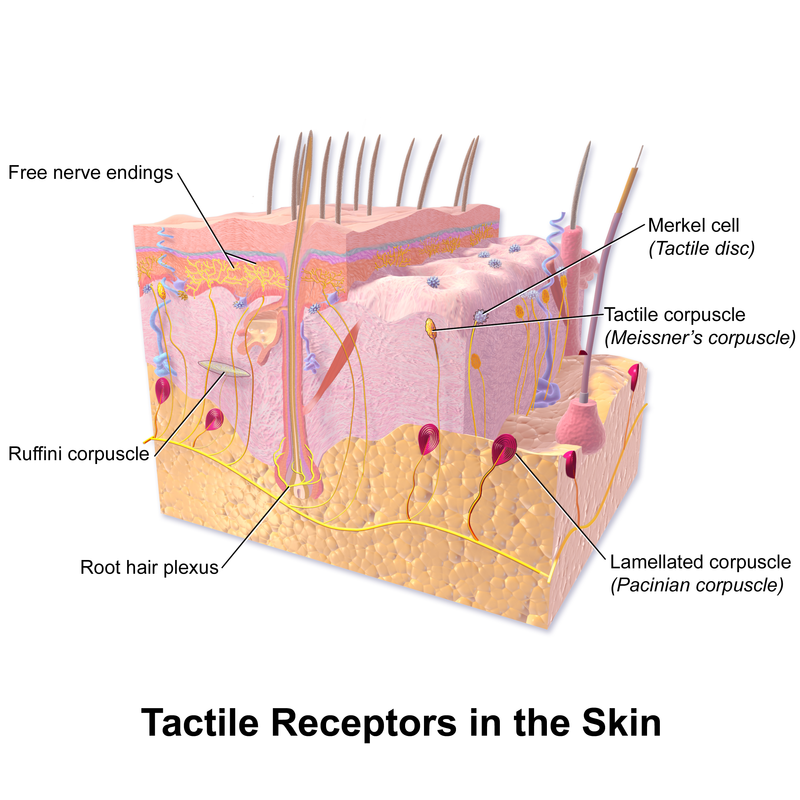
\includegraphics[width=\linewidth]{images/tactileReceptors}
\end{figure}
\end{multicols}
\end{frame}
}

\begin{frame}{La perception tactile}
\begin{table}[]
\centering
\footnotesize
	\begin{tabular}[]{lrrrr}
		\toprule
		\textbf{Nom}			& \textbf{Type}	
		                    & \textbf{Fréquence} & \textbf{Surface de} 
		                    & \textbf{Rôle} \\
		                    & & \textbf{du stimulus} & \textbf{réception} &\\
		\midrule
		Disques de Merkel				& SA-I	& 0-10Hz	& Restreint & Rebord, Pression		\\[0.25em]
		Corp. de Ruffini				& SA-II	& 0-10Hz	& Large & Etirement de la peau	\\[0.25em]
		Corp. de Meissner					& FA-I	& 20-50Hz	& Restreint & Pression	\\[0.25em]
		Corp. de Pacini				& FA-II	& 100-300Hz	& Large & Pression profonde,\\
		& & & & vibration\\
		\bottomrule
	\end{tabular}
	\caption{Caractéristiques des méchanorécepteurs}
\end{table}
\end{frame}

{
\setbeamertemplate{frame footer}{\copyright http://www.ib.cnea.gov.ar}
\begin{frame}{La perception tactile}
\begin{figure}
\centering
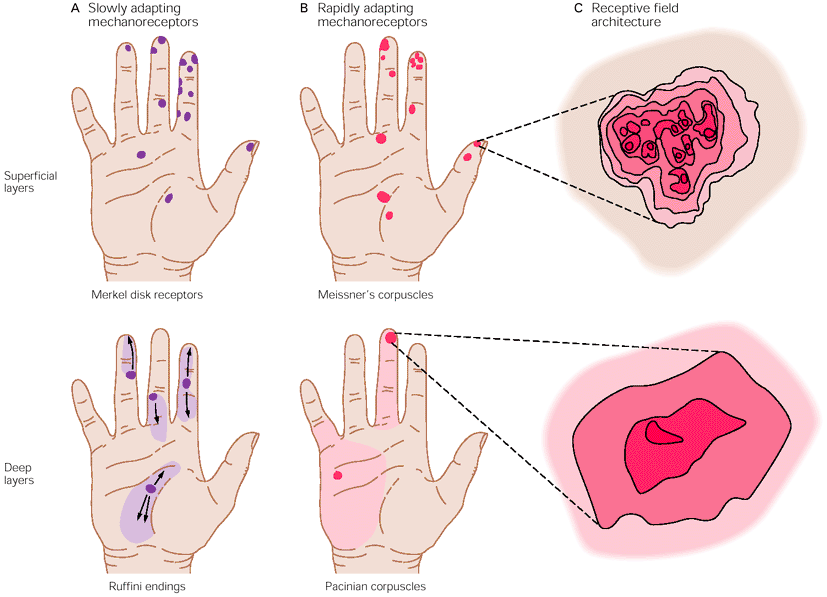
\includegraphics[width=10cm]{images/mechanoreceptors}
\end{figure}
\end{frame}
}
%\note{
%	\begin{itemize}
%		\item Splitshow (Mac OS X)\\\url{https://code.google.com/p/splitshow/}
%		\item pdf-presenter (Windows)\\\url{https://code.google.com/p/pdf-presenter/}
%	\end{itemize} 
%}

{
\setbeamertemplate{frame footer}{\cite{mancini2014whole}}
\begin{frame}{La perception tactile}
\begin{figure}
\centering
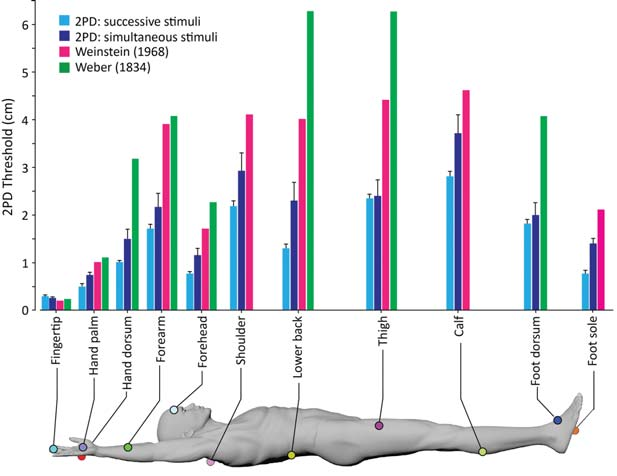
\includegraphics[width=8cm]{images/tactile_acuity}
\end{figure}
\end{frame}
}

{
\setbeamertemplate{frame footer}{\copyright Wikipedia.org}
\begin{frame}{La perception tactile - thermique}
\begin{itemize}
\item Récepteurs thermiques identifiés récemment (Nobel 2021)
\item Les récepteurs mesurent les variations de températures
\begin{itemize}
\item récepteurs au chaud (entre 30 et 46 $^{\circ}C$)
\item récepteurs au froid (entre 10 et 35 $^{\circ}C$)
\end{itemize}
\end{itemize}
\begin{figure}
\centering
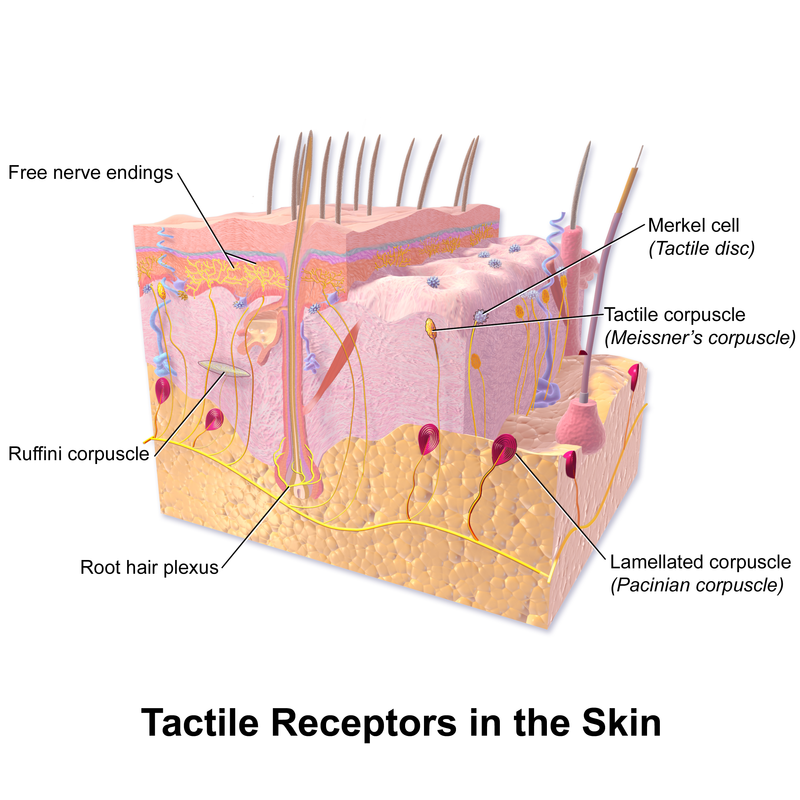
\includegraphics[width=4cm]{images/tactileReceptors}
\end{figure}
\end{frame}
}

\subsection{Illusions tactiles}
{
\setbeamertemplate{frame footer}{\cite{Hayward2008b}}
\begin{frame}{Illusions tactiles}
\begin{figure}
\centering
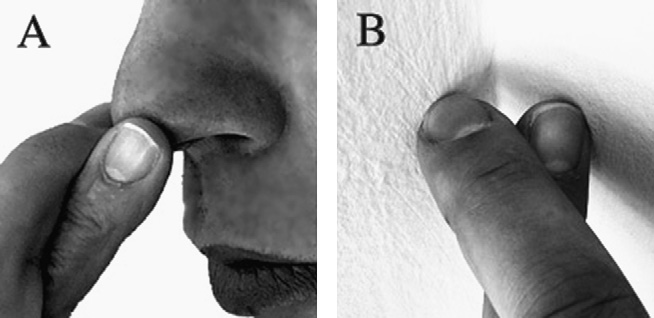
\includegraphics[width=8cm]{images/illusions_aristote}
\caption{Illusion d'Aristote. Lorsque les doigts sont croisés, deux surfaces sont perçues au lieu d'une (A). L'illusion inverse consiste à ne ressentir qu'une surface au lieu de deux (B).}
\end{figure}
\end{frame}

\begin{frame}{Illusions tactiles}
\begin{figure}
\centering
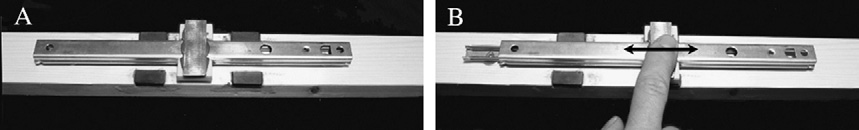
\includegraphics[width=\linewidth]{images/illusions_bump}
\caption{Illusion de bosses et creux. Réalisée avec une glissière et des aimants. Les aimants vont réduire la vitesse de déplacement de la glissière, induisant une illusion de bosses et de creux.}
\end{figure}
\end{frame}
}

{
\setbeamertemplate{frame footer}{\cite{Tan1997c}}
\begin{frame}{Illusions tactiles}
\begin{figure}
\centering
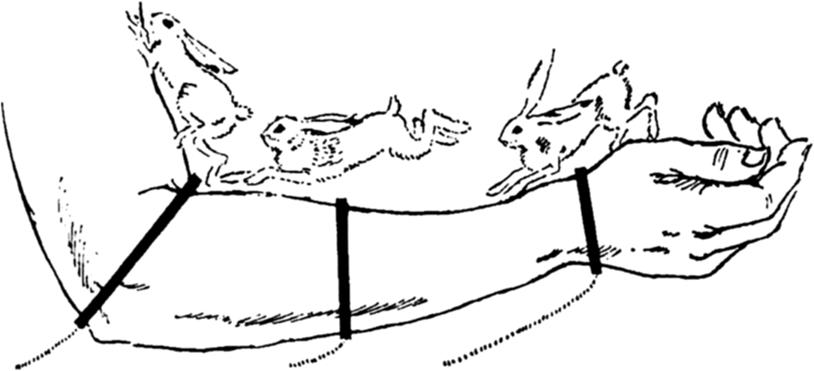
\includegraphics[width=10cm]{images/illusions_rabbit}
\caption{"Cutaneous rabbit illusion". Lorsque 3 vibrations sont appliquées successivement sur la surface de la peau, seul un stimulus continu est ressenti.}
\end{figure}
\end{frame}
}

{
\setbeamertemplate{frame footer}{\cite{Salzer2007}}
\begin{frame}{Illusions tactiles}
\begin{figure}
\centering
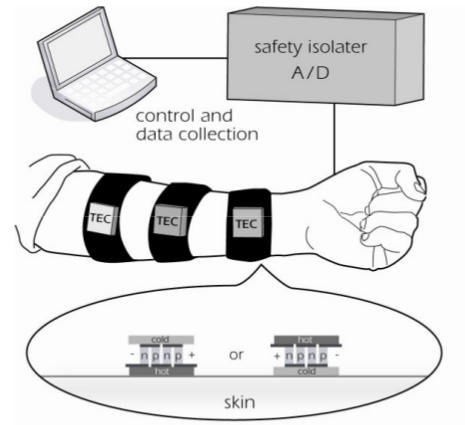
\includegraphics[width=5cm]{images/thermalgrill}
\caption{Illusion du grill. Stimuli chauds (40$^{\circ}C$) et froids (20$^{\circ}C$) appliqués successivement sur la peau. Une sensation de brûlure apparait.}
\end{figure}
\end{frame}
}

\subsection{Interfaces Tactile}
\begin{frame}{Interfaces tactiles - Contact}
\begin{itemize}
\item Vibreurs
\item Solénoïdes
\end{itemize}

\begin{multicols}{2}
\begin{figure}
\centering
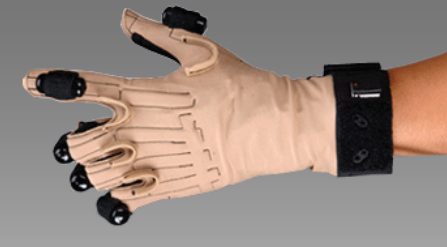
\includegraphics[width=3cm]{images/cybertouch}
\caption{\copyright Cybertouch.com}
\end{figure}
%\movie[externalviewer]{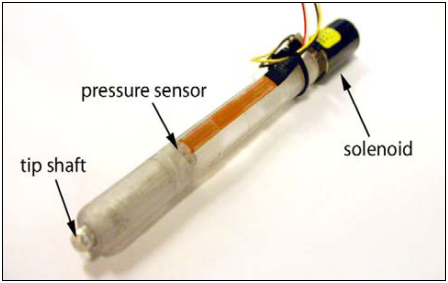
\includegraphics[width=4cm]{images/hapticPen.PNG}}{videos/Haptic_Pen.mp4}
%\includemovie[poster,text={\small(Loading Circle-m-increase3.mp4)}]{4cm}{4cm}{videos/Haptic_Pen.mp4}
\begin{figure}
\centering
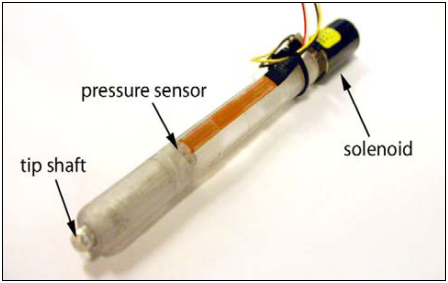
\includegraphics[width=3cm]{images/hapticPen}
\vspace{-0.2cm}
\caption{\cite{Lee2004}}
\end{figure}
\end{multicols}

\vspace{-1cm}

\begin{figure}
\centering
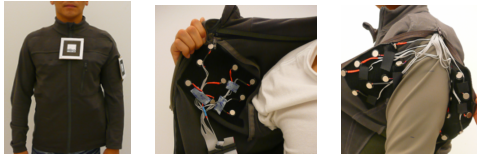
\includegraphics[width=8cm]{images/Rahman2010}
\caption{\cite{Rahman2010}}
\end{figure}

\end{frame}


{
\setbeamertemplate{frame footer}{\copyright precisionmicrodrives.com}
\begin{frame}{Moteur à masse excentrique (ERM)}
\begin{figure}
\centering
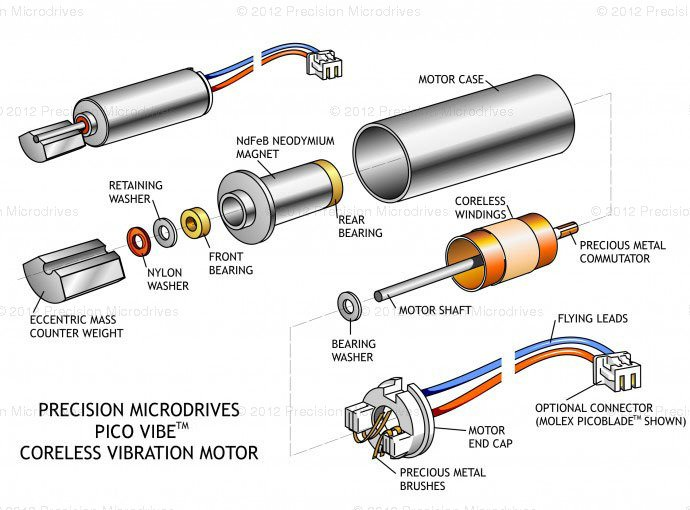
\includegraphics[width=\linewidth]{images/ERM}
\end{figure}
\end{frame}

\begin{frame}{Moteur à masse excentrique (ERM)}
\begin{figure}
\centering
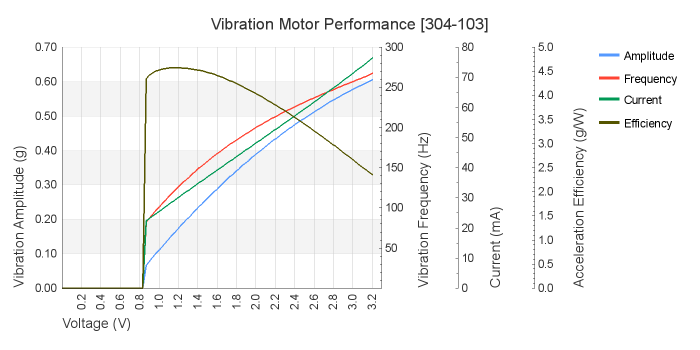
\includegraphics[width=\linewidth]{images/ERM_output}
\end{figure}
\end{frame}
}

\begin{frame}{Exemple: manette Xbox One}
\begin{figure}
\centering
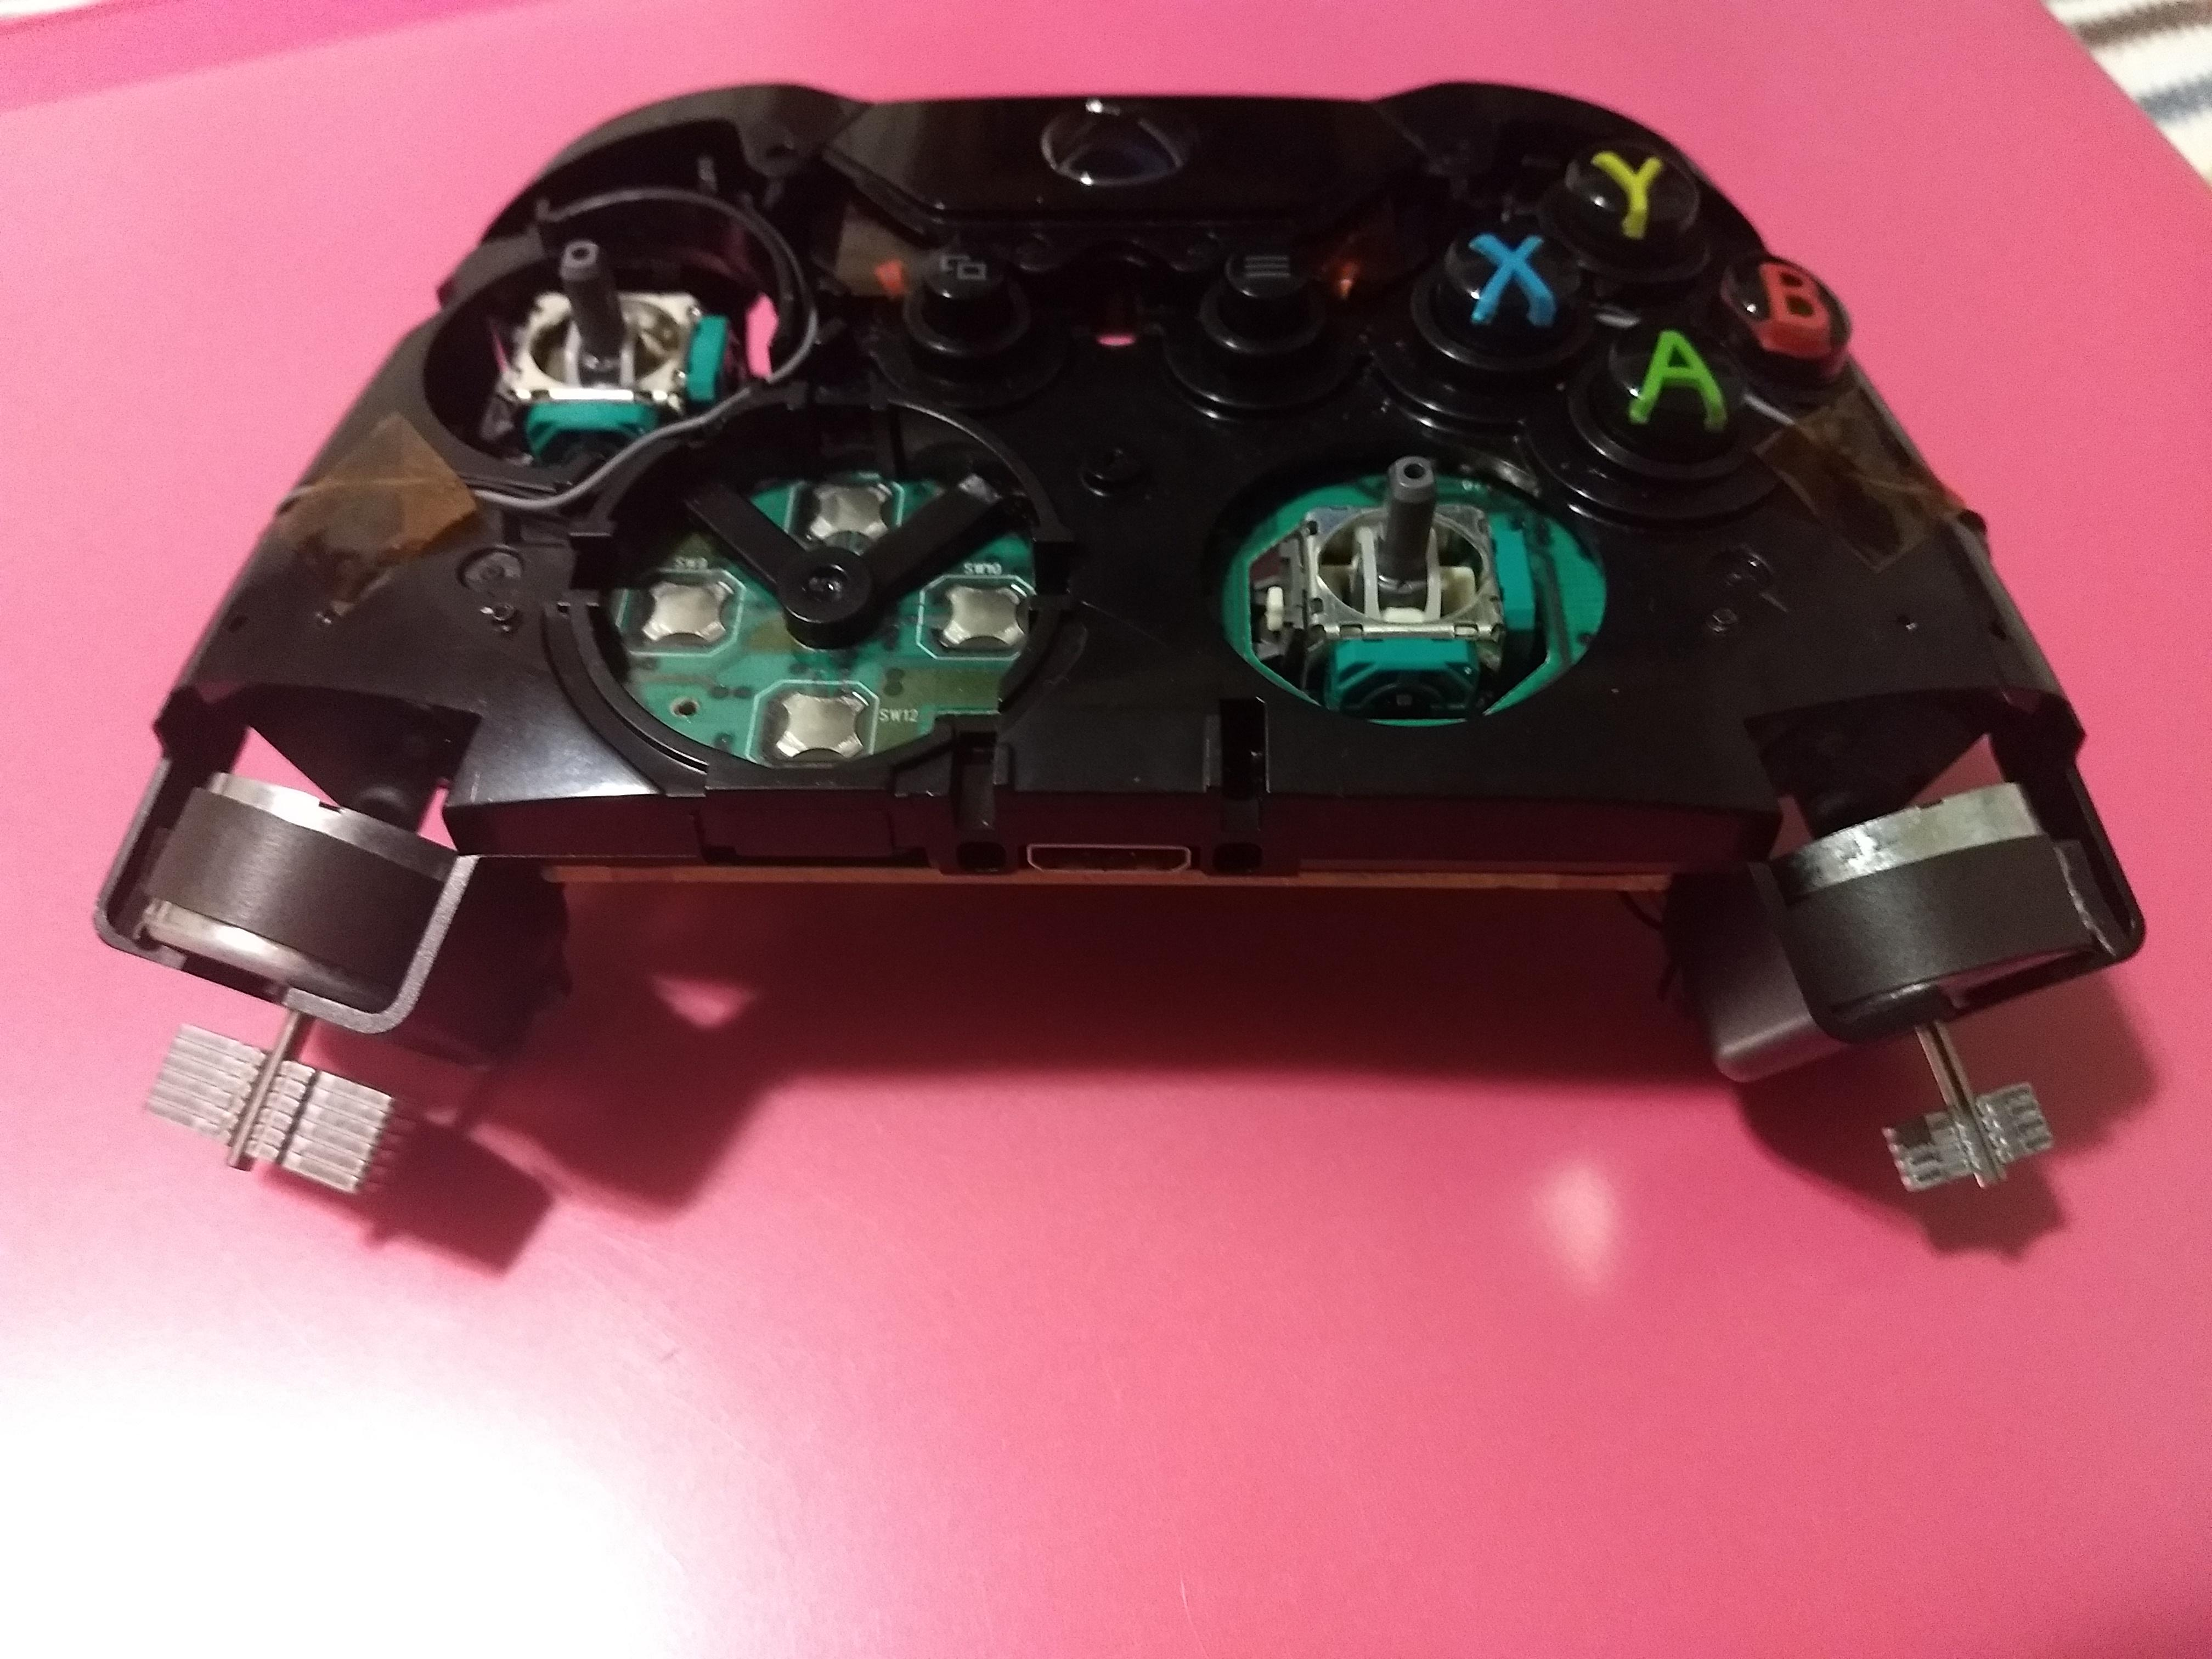
\includegraphics[width=\linewidth]{images/xboxone}
\end{figure}
\end{frame}

{
\setbeamertemplate{frame footer}{\copyright precisionmicrodrives.com}
\begin{frame}{Moteur linéaire (LRA)}
\begin{figure}
\centering
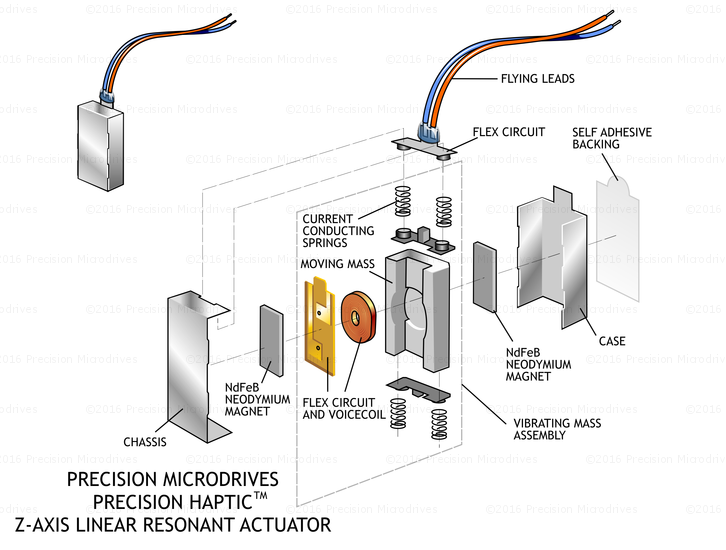
\includegraphics[width=\linewidth]{images/lra}
\end{figure}
\end{frame}

\begin{frame}{Moteur linéaire (LRA)}
\begin{figure}
\centering
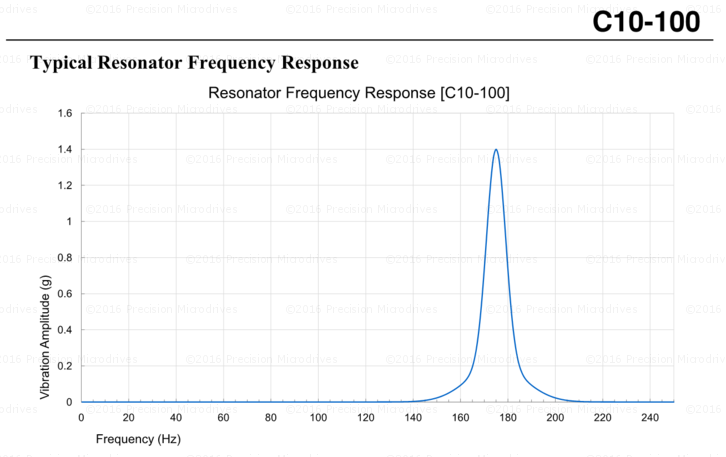
\includegraphics[width=\linewidth]{images/LRA_output}
\end{figure}
\end{frame}
}

{
\setbeamertemplate{frame footer}{\copyright ifixit.com}
\begin{frame}{Exemple: manette Switch}
\begin{figure}
\centering
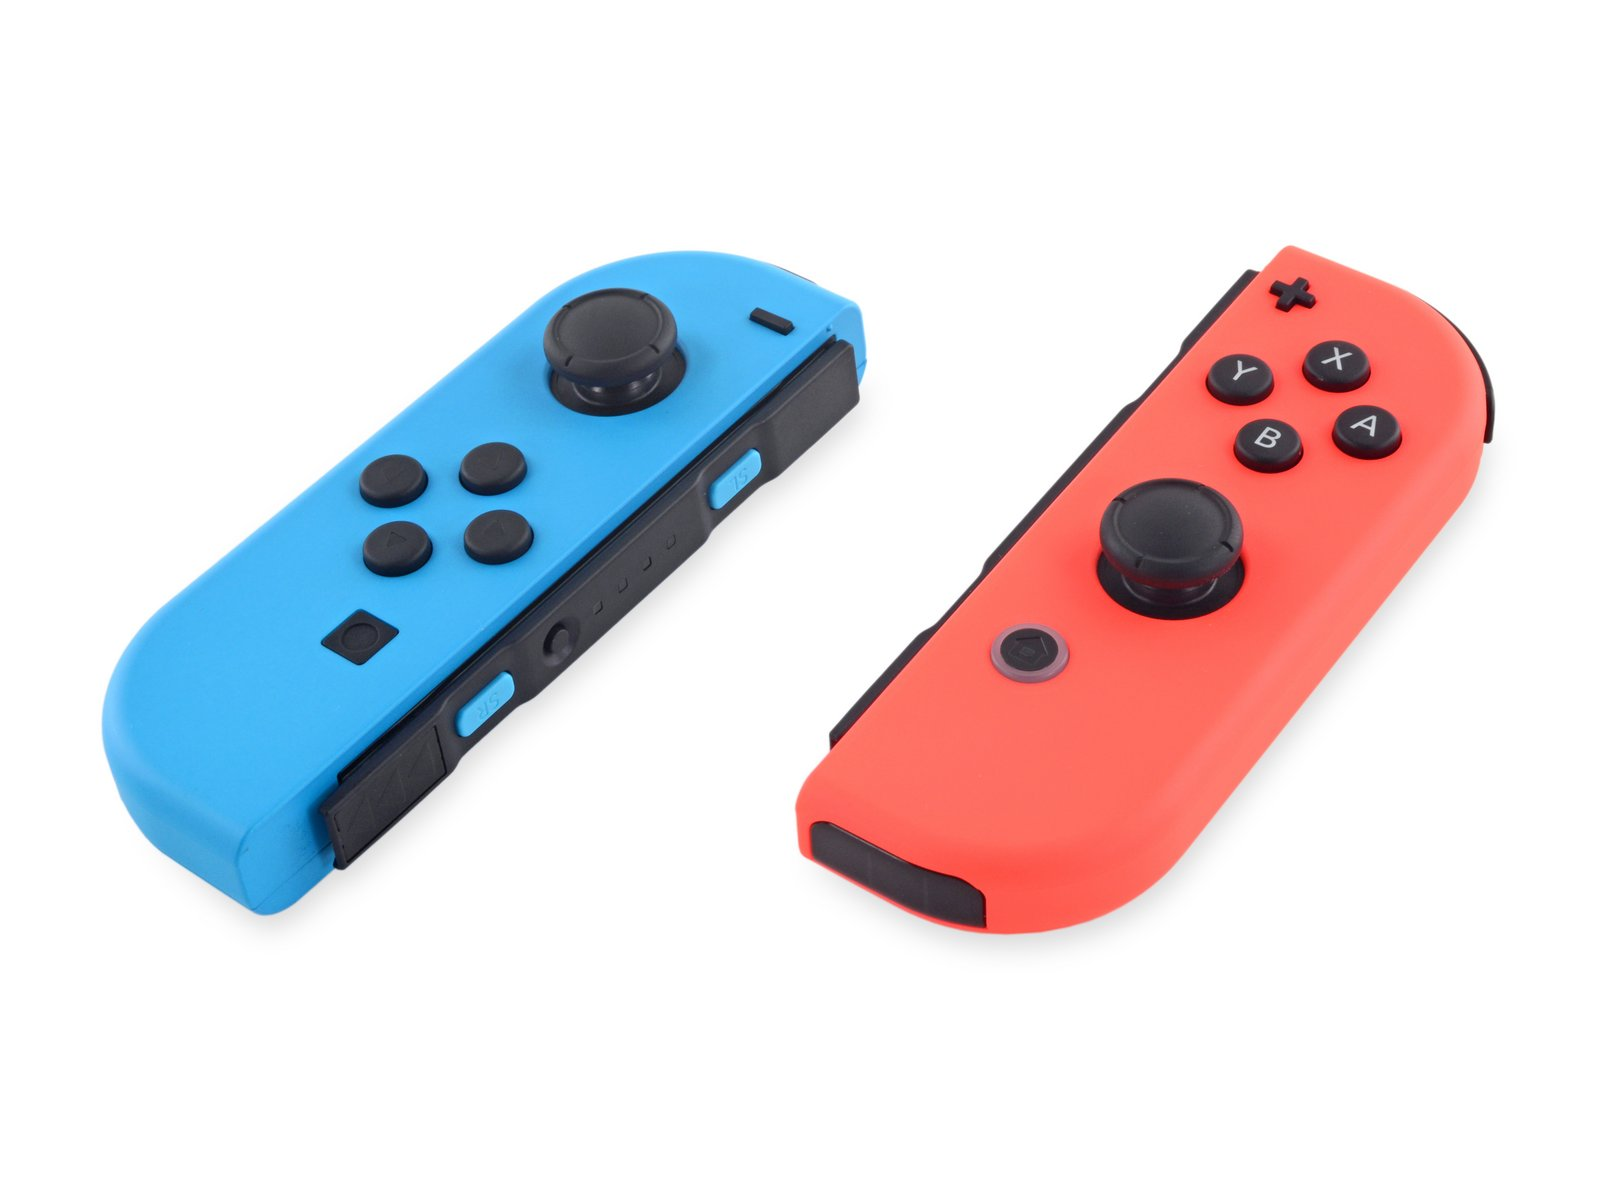
\includegraphics[width=0.4\linewidth]{images/switch1}
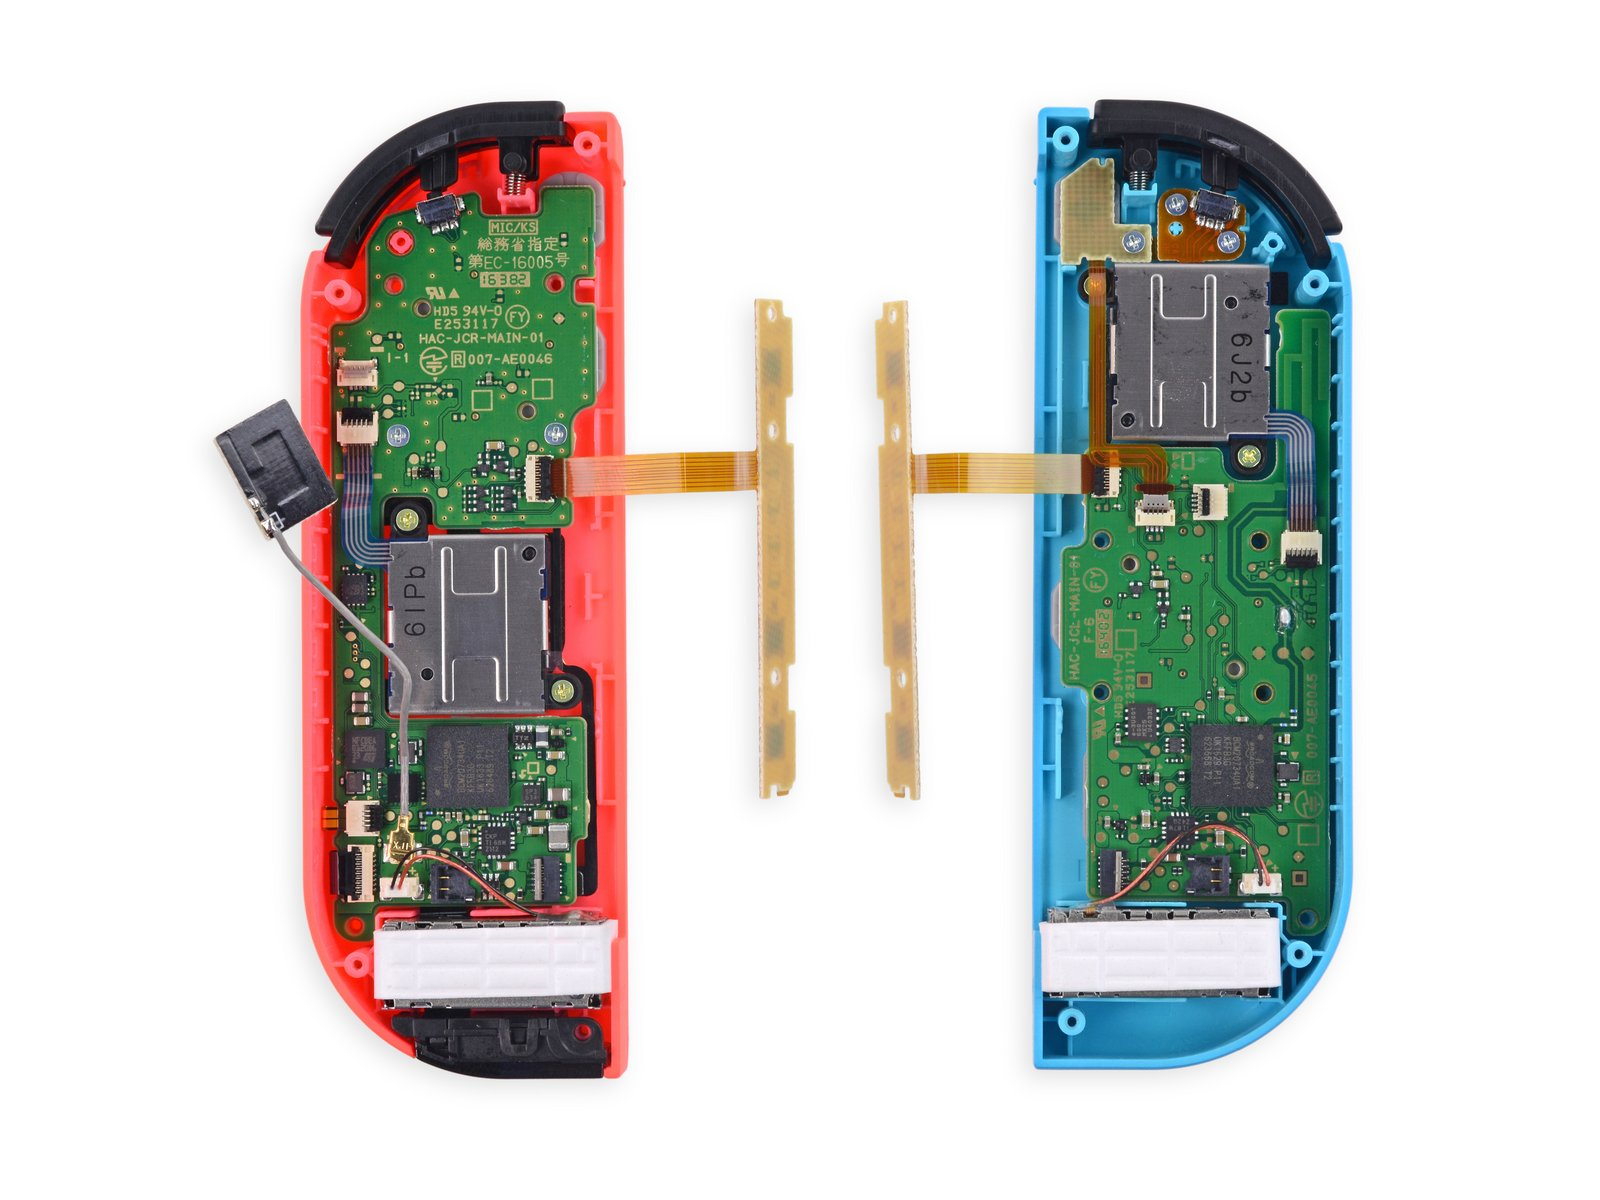
\includegraphics[width=0.4\linewidth]{images/switch2}
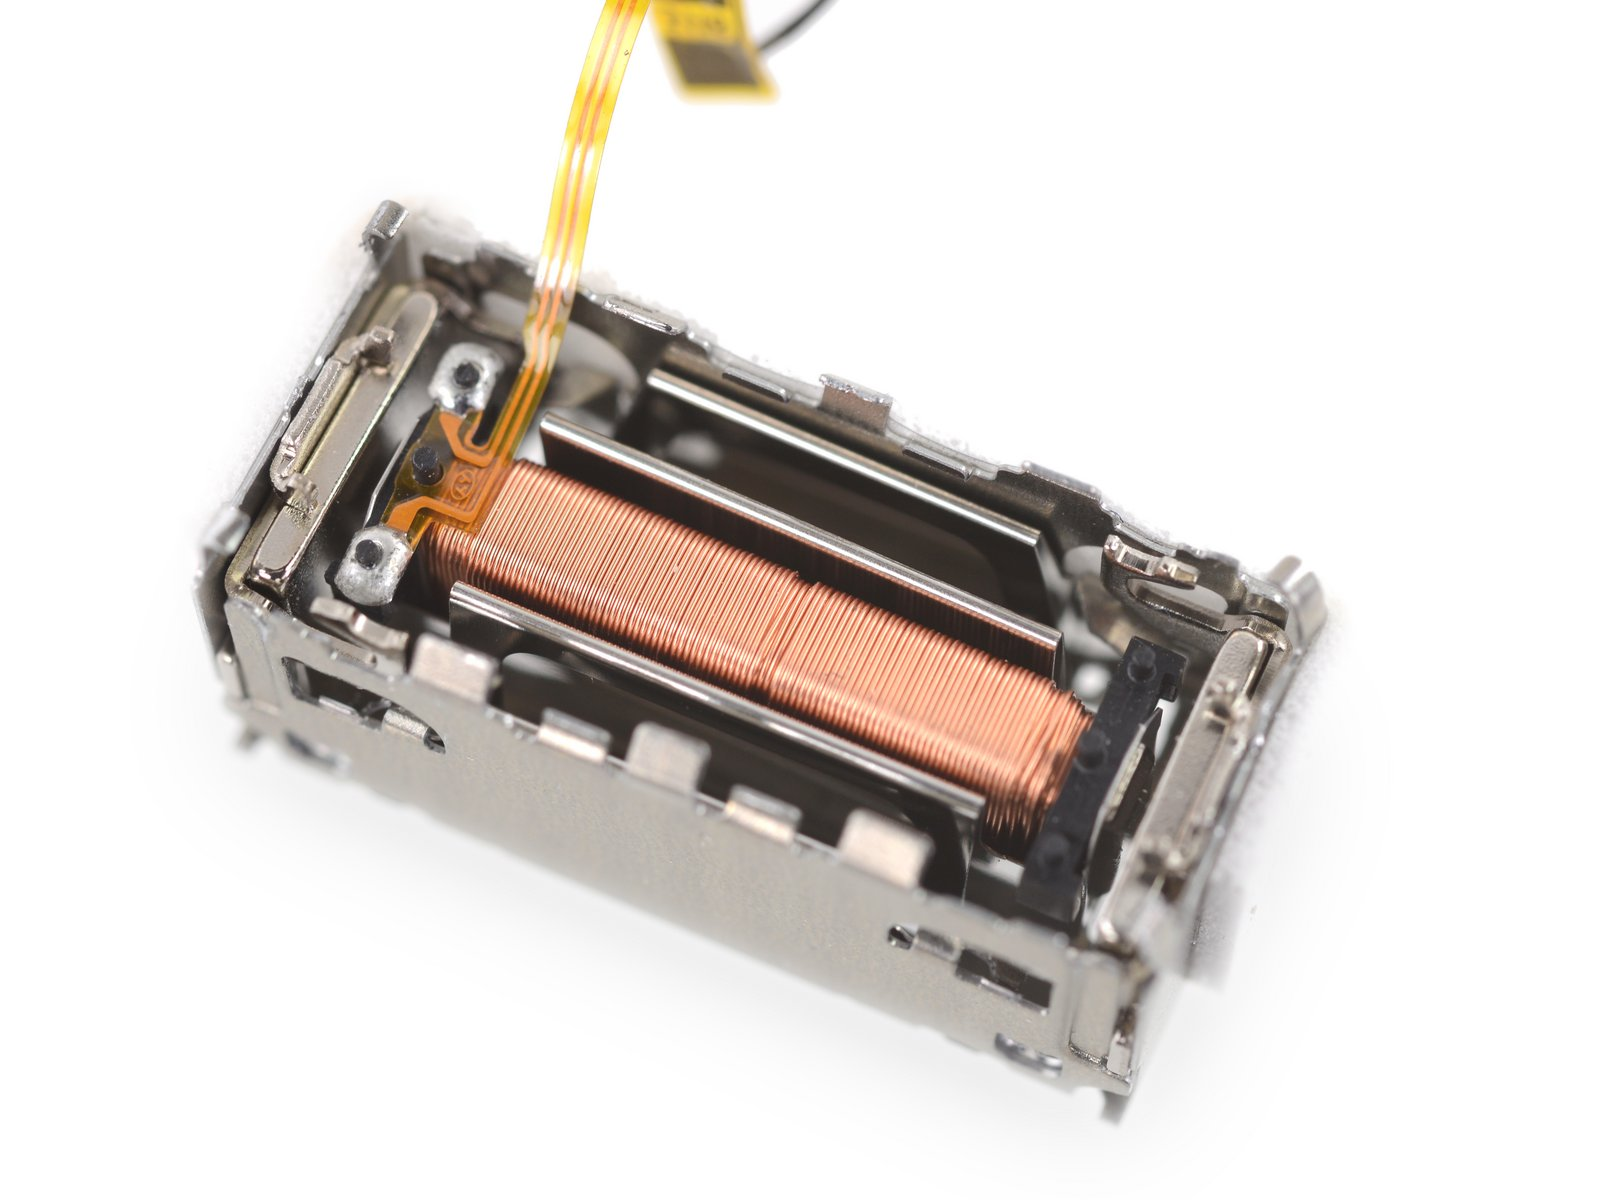
\includegraphics[width=0.4\linewidth]{images/HDRumble1}
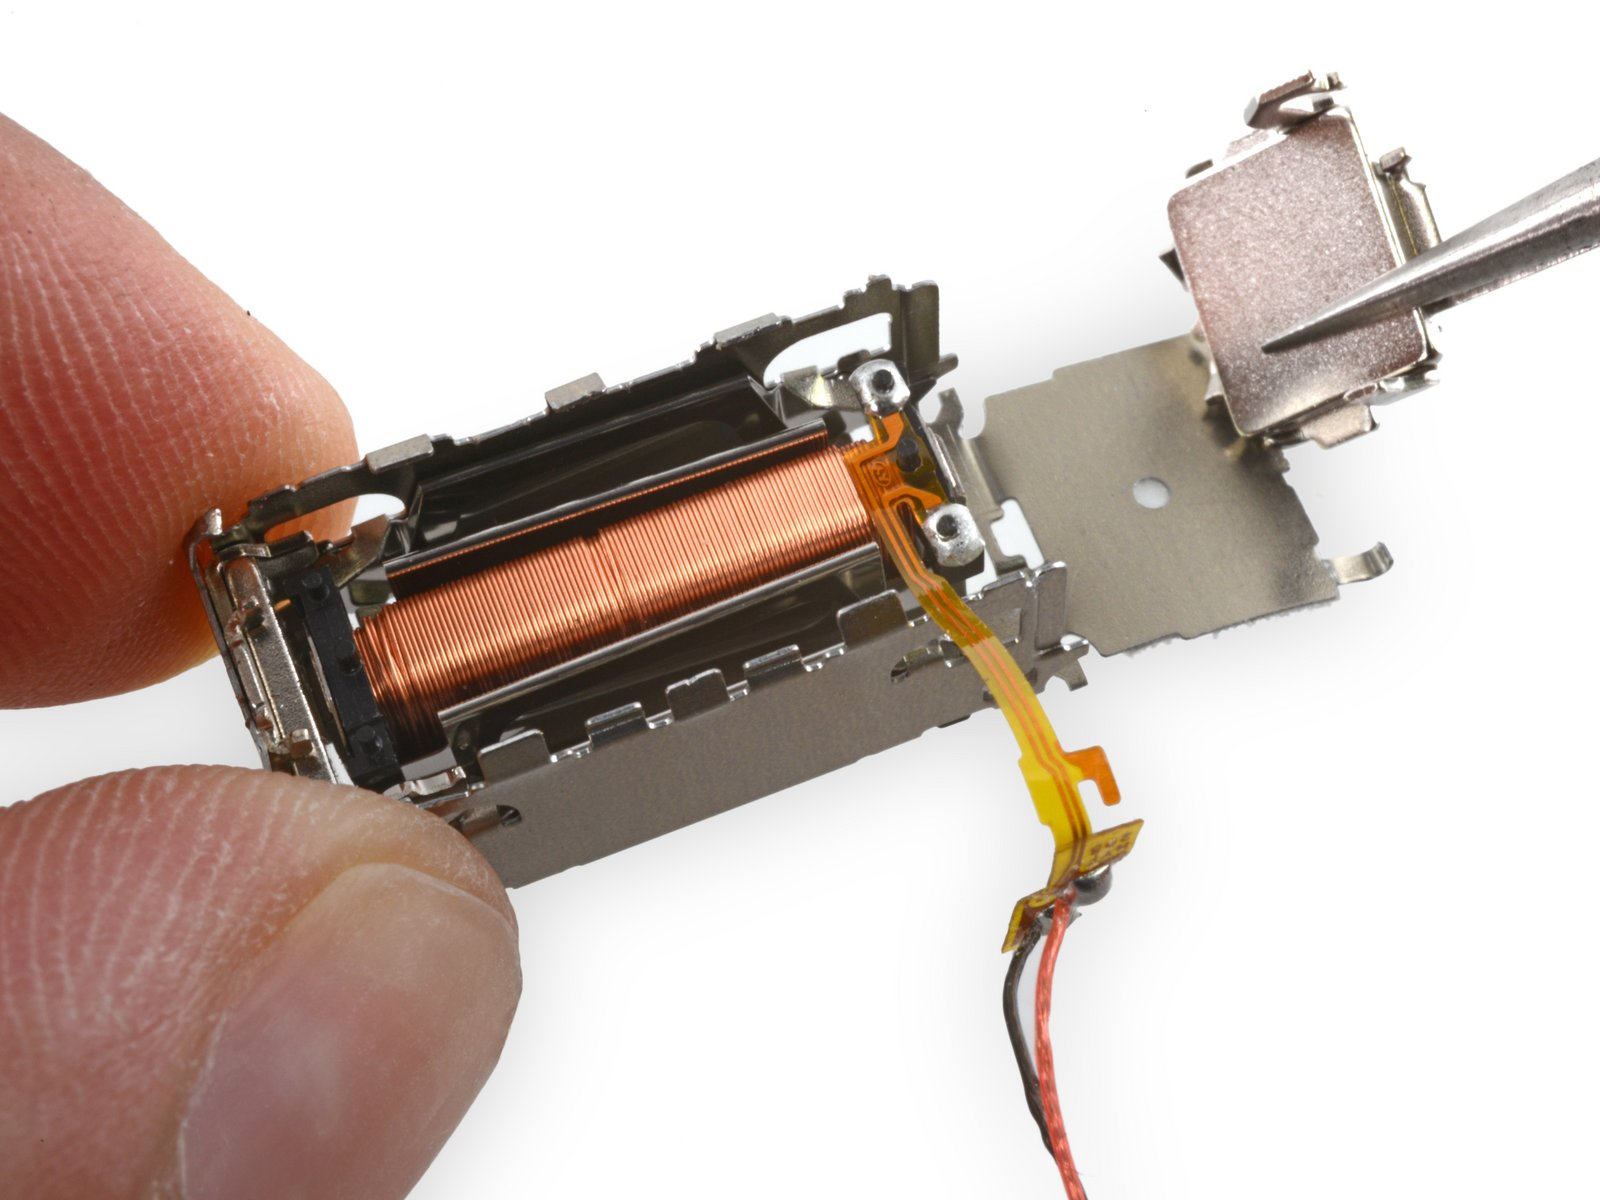
\includegraphics[width=0.4\linewidth]{images/HDRumble2}
\end{figure}
\end{frame}
}

{
\setbeamertemplate{frame footer}{\copyright actronika.com}
\begin{frame}{Voice-coil}
\begin{figure}
\centering
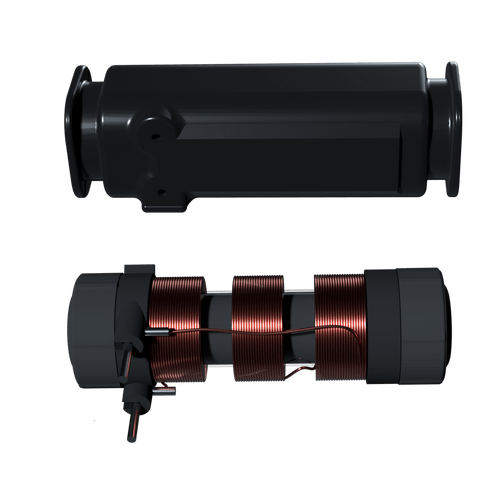
\includegraphics[width=0.45\linewidth]{images/voice-coil_2}
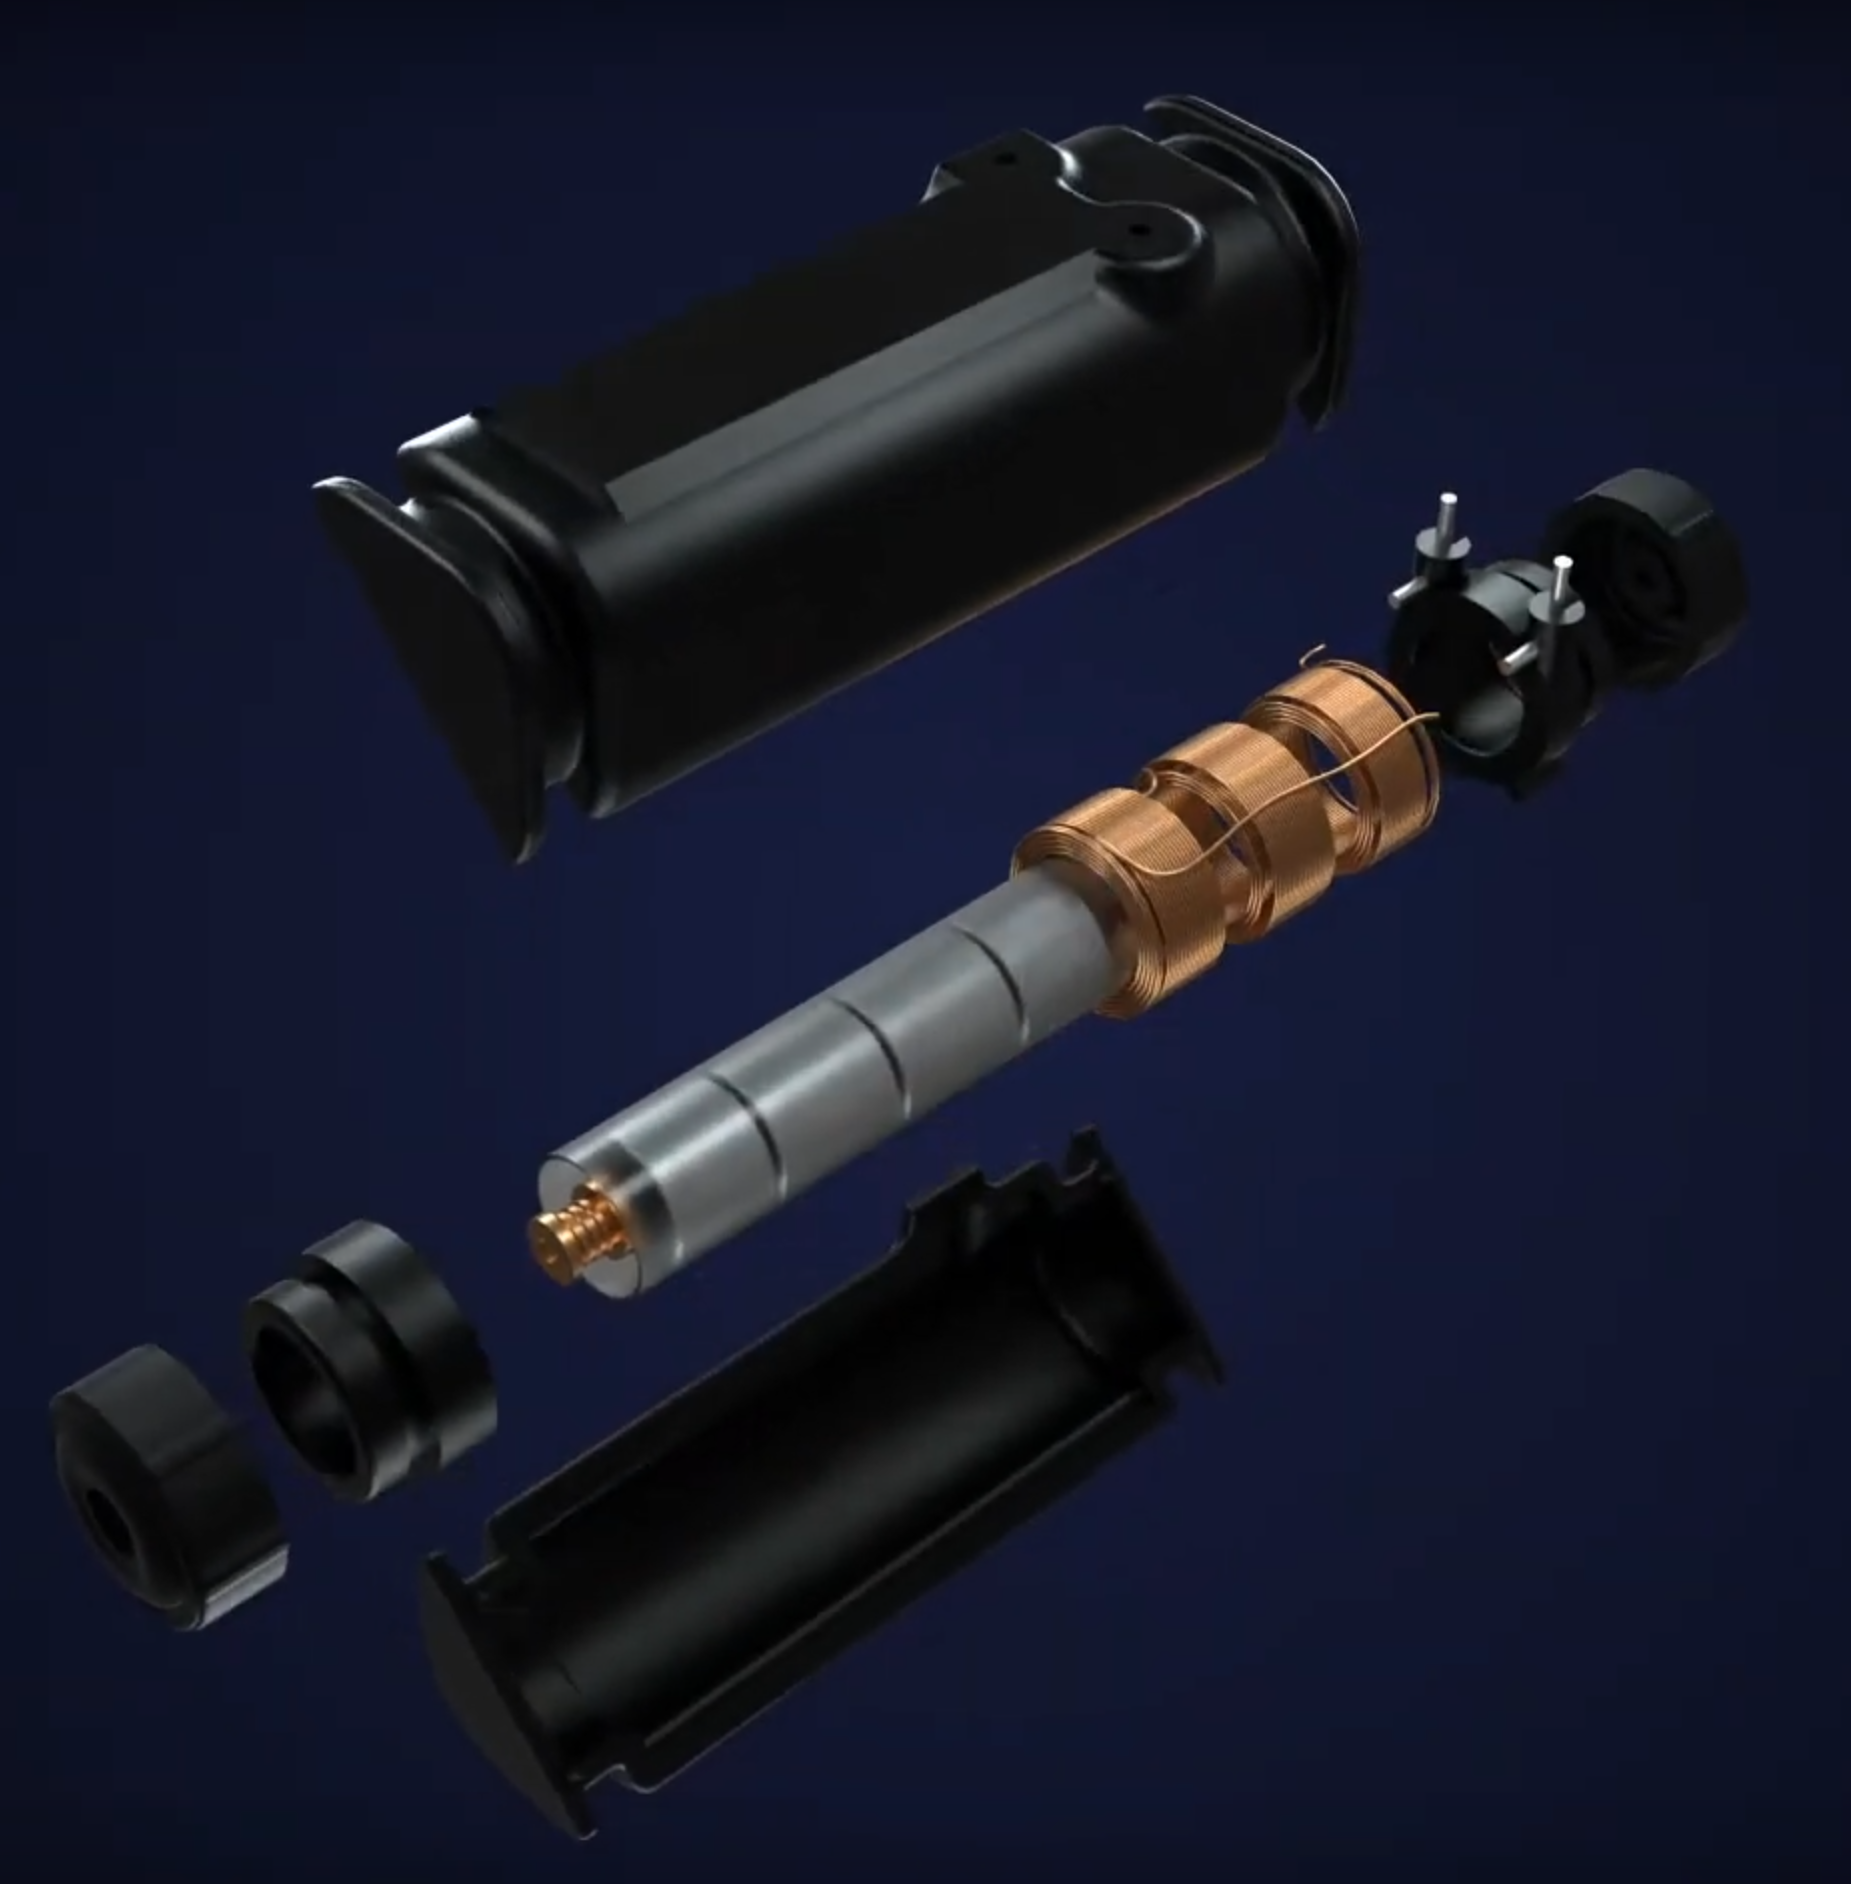
\includegraphics[width=0.45\linewidth]{images/voice-coil}
\end{figure}
\end{frame}
}

{
\setbeamertemplate{frame footer}{\copyright actronika.com}
\begin{frame}{Voice-coil}
\begin{figure}
\centering
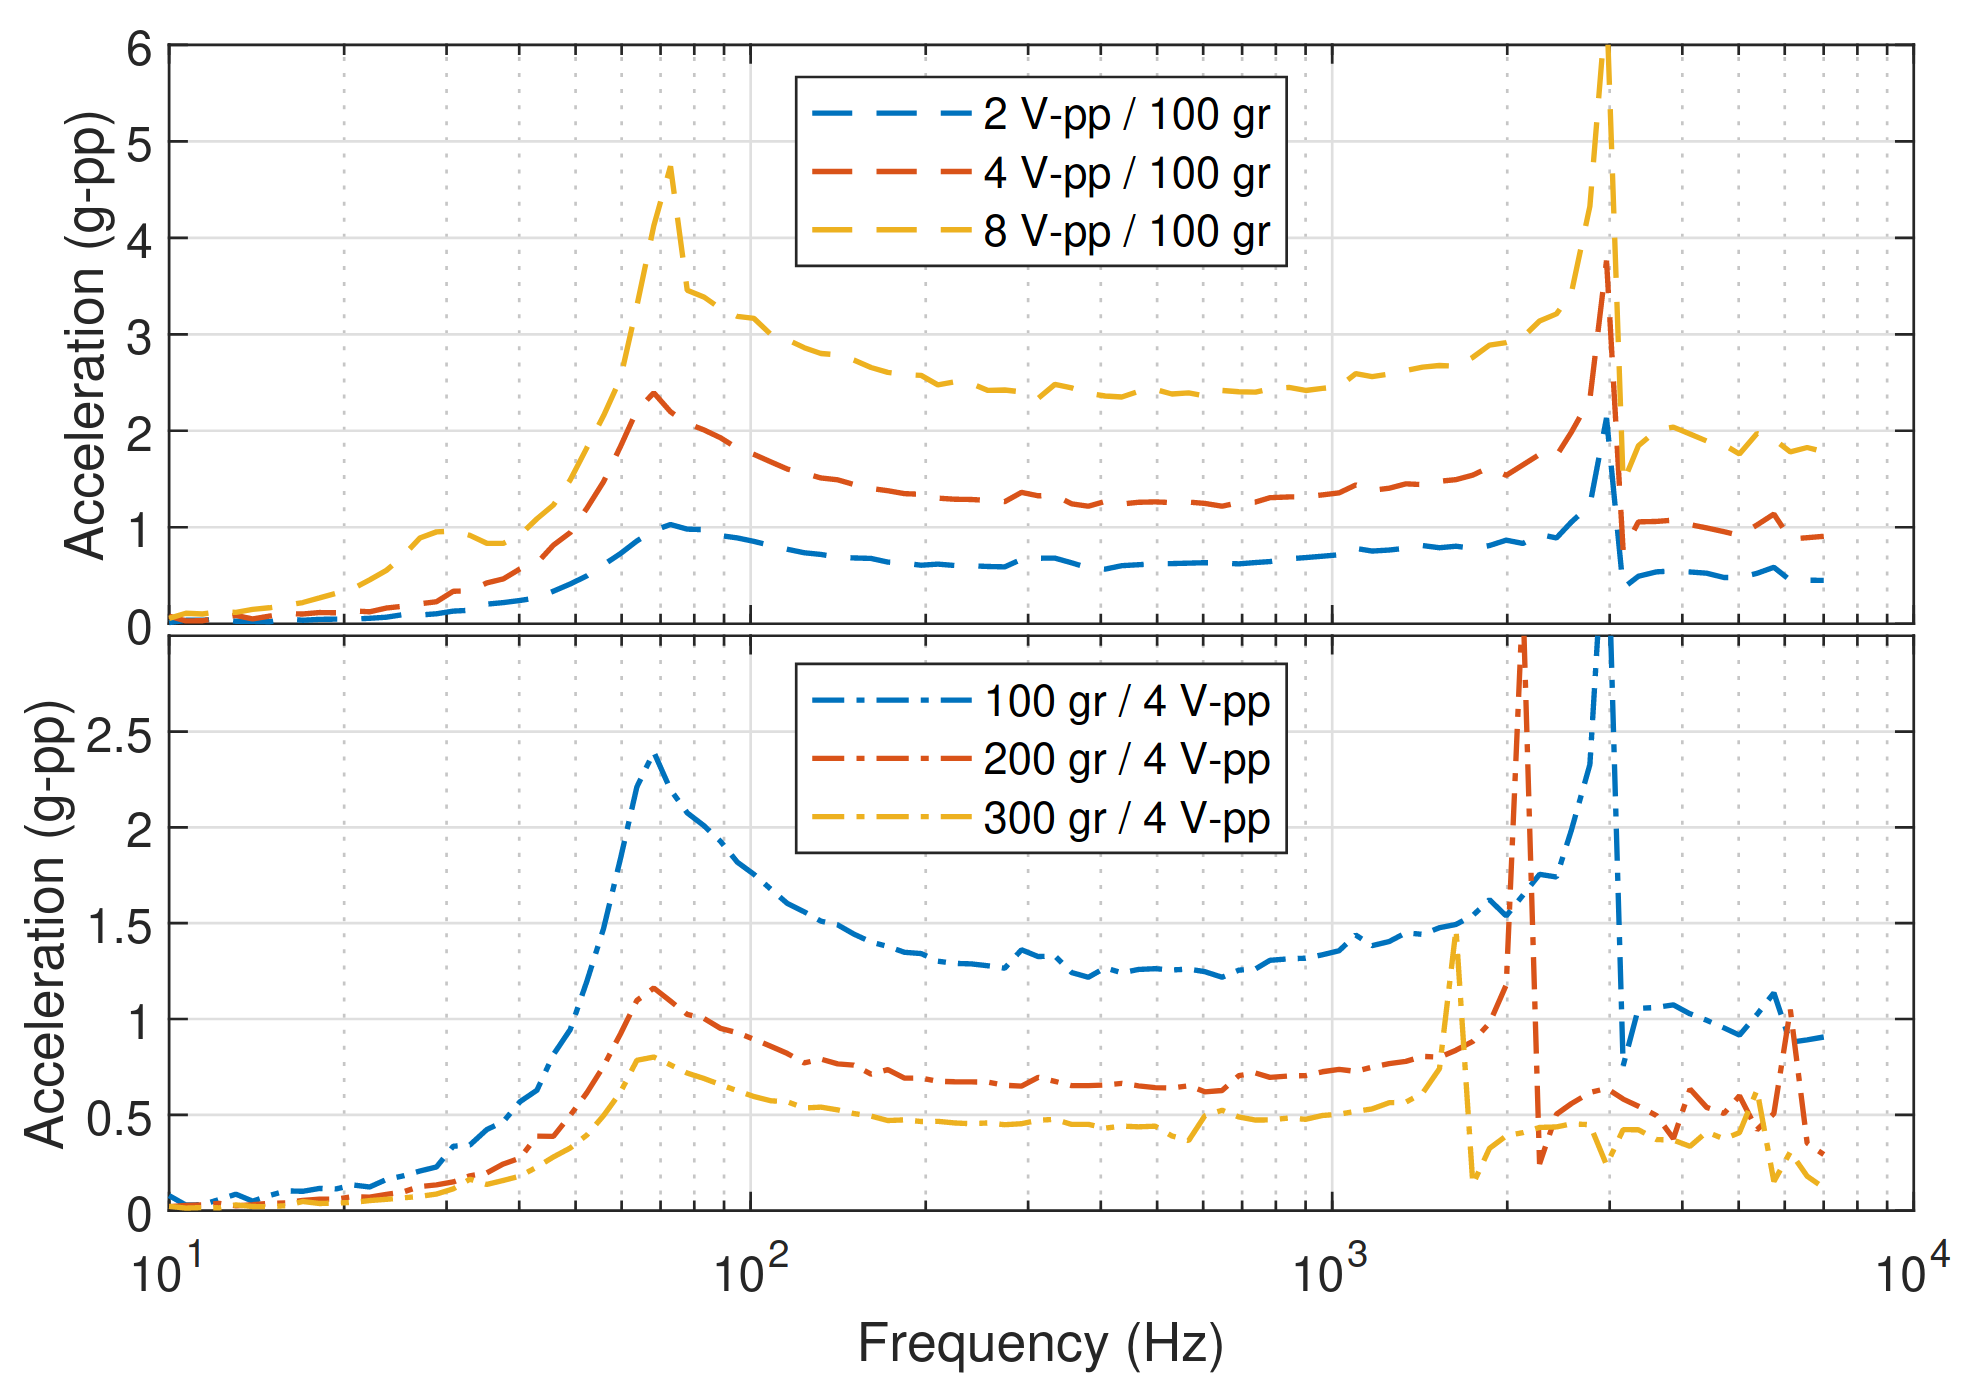
\includegraphics[width=\linewidth]{images/voice-coil_bandwidth}
\end{figure}
\end{frame}
}


{
\setbeamertemplate{frame footer}{\cite{choi2020development}}
\begin{frame}{Interfaces tactiles - Contact}
\begin{figure}
\centering
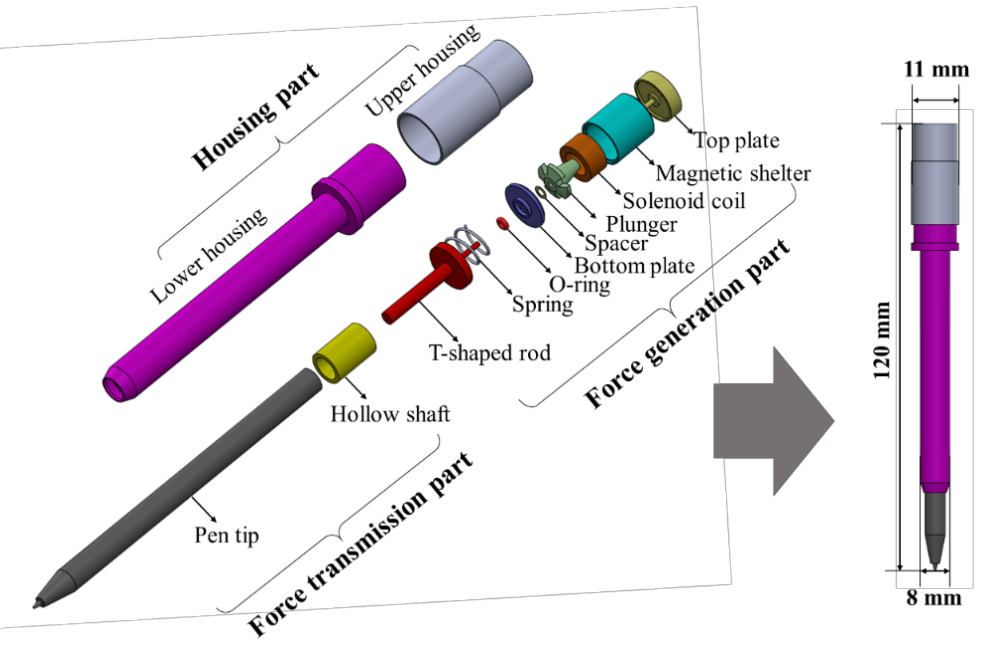
\includegraphics[width=\linewidth]{images/stylus}
\end{figure}
\end{frame}
}

{
\setbeamertemplate{frame footer}{\cite{benko2016}}
\begin{frame}{Interfaces tactiles - Contact}
\begin{figure}
\href{run:videos/microsoft_texture.mp4}{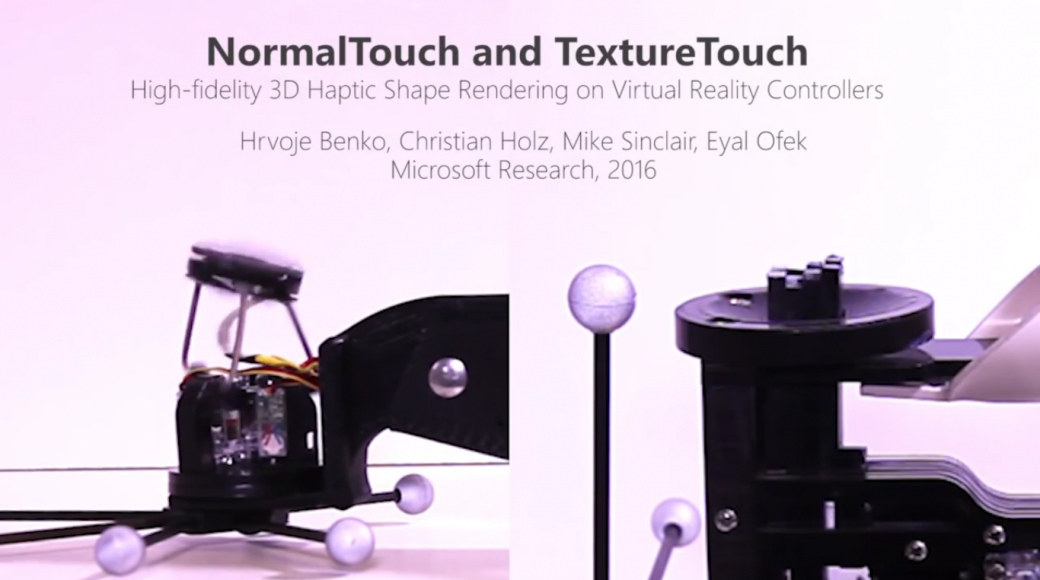
\includegraphics[width=\linewidth]{images/microsoft_textureTouch}}
\end{figure}

\end{frame}
}

{
\setbeamertemplate{frame footer}{\copyright ifixit.com}
\begin{frame}{Exemple: manette PS5}
\begin{figure}
\centering
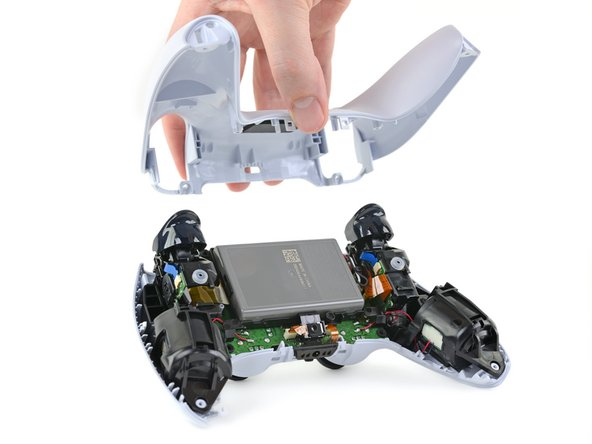
\includegraphics[width=0.4\linewidth]{images/ps5_open}
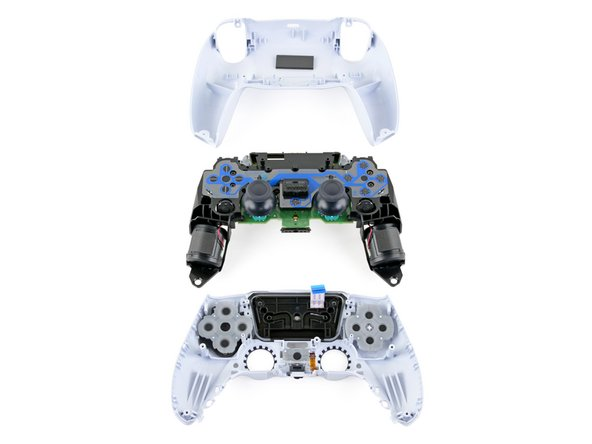
\includegraphics[width=0.4\linewidth]{images/ps5_breakdown}
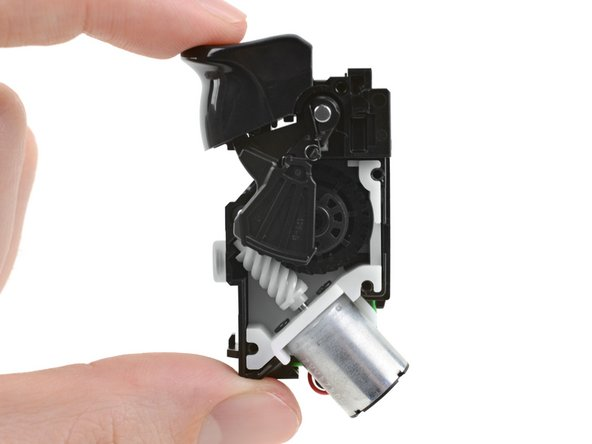
\includegraphics[width=0.4\linewidth]{images/ps5_trigger}
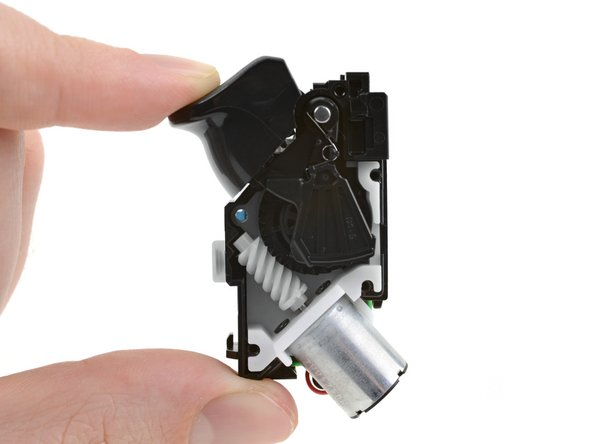
\includegraphics[width=0.4\linewidth]{images/ps5_trigger2}
\end{figure}
\end{frame}
}

\begin{frame}{Interfaces tactiles - Texture}
\begin{multicols}{2}

\begin{itemize}
\item Matrice de picots
\item Actuateur piezo-electrique
\item Vibration electrostatique
\end{itemize}

\begin{figure}
\centering
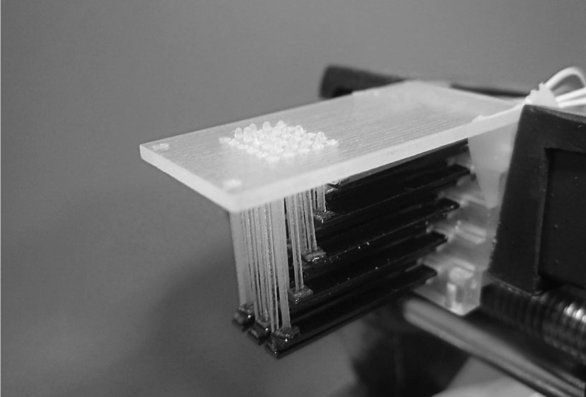
\includegraphics[width=4cm]{images/texture}
\caption{\cite{Yang2008}}
\end{figure}

\begin{figure}
\centering
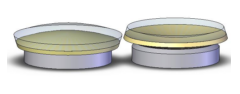
\includegraphics[width=4cm]{images/piezo}
\end{figure}

%\vspace{-1cm}
\begin{figure}
\centering
%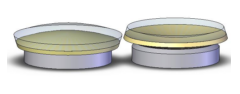
\includegraphics[width=4cm]{images/piezo}
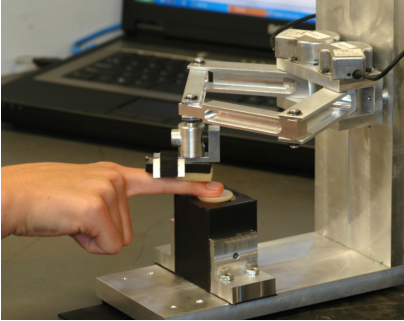
\includegraphics[width=4cm]{images/piezo2}
\caption{\cite{Winfield2007}}
\end{figure}

\end{multicols}

%\vspace{-0.5cm}
%\begin{figure}
%\centering
%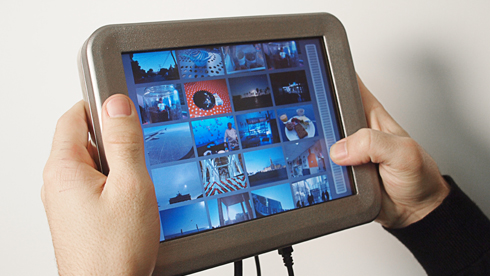
\includegraphics[width=4cm]{images/teslatouch-03}
%\caption{\cite{bau2010}}
%\end{figure}

%\begin{figure}
%\centering
%\movie[externalviewer]{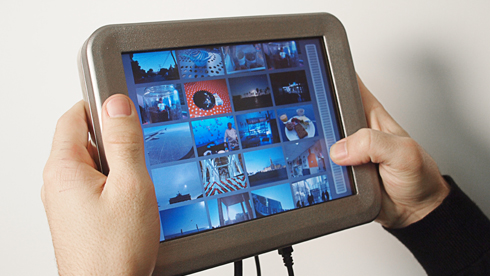
\includegraphics[width=4cm]{images/teslatouch-03}}{videos/TeslaTouch.mov}
%\linebreak
%
\includegraphics[width=\linewidth]{images/none}{\copyright \mbox{Bau et al., 2010}}
%\end{figure}


\end{frame}

{
\setbeamertemplate{frame footer}{\cite{bau2010}}
\begin{frame}{Interfaces tactiles - Texture}
\begin{figure}
\href{run:videos/TeslaTouch.mov}{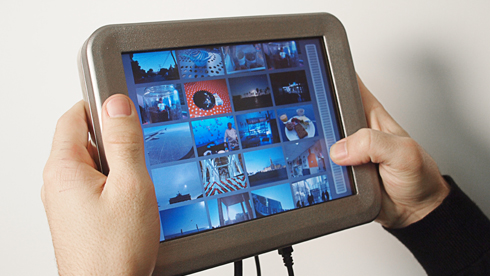
\includegraphics[width=\linewidth]{images/teslatouch-03}}
\end{figure}
\end{frame}
}

\begin{frame}{Interfaces tactiles - pression sans contact}
\begin{multicols}{2}

\begin{itemize}
\item Ultrasonic transmitters array
\item Projecteur de flux d'air
\end{itemize}

\begin{figure}
\centering
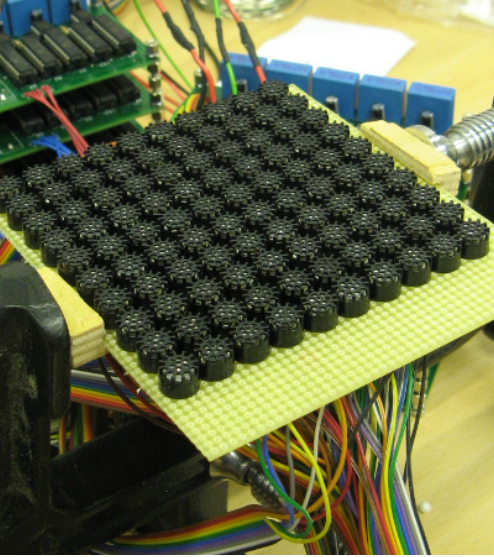
\includegraphics[width=2.25cm]{images/ultrahaptics}
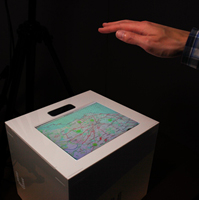
\includegraphics[width=2.5cm]{images/ultrahaptics_project_photo}
\caption{\cite{Alexander2011}}
\end{figure}

%\begin{figure}
%\centering
%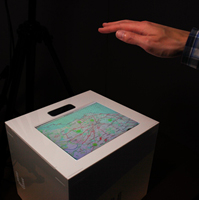
\includegraphics[width=2cm]{images/ultrahaptics_project_photo}
%\end{figure}

\begin{figure}
\centering
\includegraphics[width=4cm]{images/AIREALVortexRingFig}
%\caption{\cite{Sodhi2013}}
%\includegraphics[width=4cm]{images/AIREALVortexRingFig}{}
\end{figure}
\vspace{-1.5cm}
\begin{figure}
\includegraphics[width=4cm]{images/aireal2}
\caption{\cite{Sodhi2013}}
\end{figure}

\end{multicols}
\end{frame}

{
\setbeamertemplate{frame footer}{\cite{Sodhi2013}}
\begin{frame}{Interfaces tactiles - Pression sans contact}
\begin{figure}
\href{run:videos/Aireal.mp4}{\includegraphics[width=\linewidth]{images/AIREALVortexRingFig}}
\end{figure}
\end{frame}
}

\begin{frame}{Interfaces tactiles - thermique}
\begin{multicols}{2}

\begin{itemize}
\item Ventilateur + source de chaleur
\item Module Peltier
\end{itemize}

\begin{figure}
\centering
\includegraphics[width=\linewidth]{images/thermalFeedback}\caption{\cite{Dionisio1997}}
\end{figure}

\begin{figure}
\centering
\includegraphics[width=4cm]{images/peltier}
\end{figure}

\begin{figure}
\centering
\includegraphics[width=4cm]{images/katII}
\caption{\cite{Yang2008}}
\end{figure}

\end{multicols}
\end{frame}

{
\setbeamertemplate{frame footer}{\copyright Wikipedia.org}
\begin{frame}{Effet Peltier}
\begin{itemize}
\item Le passage du courant dans les semi-conducteurs N et P provoquent un flux thermique
\item Découvert en 1834 par Jean-Charles Peltier
\end{itemize}
\begin{figure}
\centering
\includegraphics[width=5cm]{images/peltierEffect}
\includegraphics[width=5cm]{images/schematic-diagram-of-peltier-module}
\end{figure}
\end{frame}
}

\subsection{Rendu tactile}
\begin{frame}{Rendu tactile}
\begin{itemize}
\item Contrôle simple la plupart des cas (ex: 1 vibreur)
\begin{figure}
\centering
\includegraphics[width=\linewidth]{images/schema_haptique2}{}
\end{figure}
\item Comment rendre un effet tactile continu dans l'espace avec un nombre limité de vibreurs?
\end{itemize}
\begin{itemize}
\item Exemple : Tactile Brush Algorithm \cite{Israr2011}
\end{itemize}
\begin{figure}
\centering
\includegraphics[width=5cm]{images/immersive-tactile-experiences}
\includegraphics[width=5cm]{images/tactile-brush-algorithm}
%{\cite{Israr2011}}
\end{figure}
\end{frame}

{
\setbeamertemplate{frame footer}{\cite{Israr2011}}
\begin{frame}{Rendu tactile - Tactile Brush Algorithm}
\begin{multicols}{2}
\begin{itemize}
\item Basé sur 2 illusions
\begin{itemize}
\item Apparent tactile motion
\begin{itemize}
\item $SOA = 0.32d + 47.3$
\end{itemize}
\item Phantom tactile sensation
\begin{itemize}
\item $A_1 = \sqrt{1-\beta}.A_v$
\item $A_2 = \sqrt{\beta}.A_v$
\item $\beta = \frac{a}{b}$ 
\end{itemize}
\end{itemize}
\end{itemize}

\begin{figure}
\centering
\includegraphics[width=5cm]{images/tactile-illusions}
\end{figure}
\end{multicols}
\end{frame}

\begin{frame}{Rendu tactile - Tactile Brush Algorithm}
\begin{figure}
\centering
\includegraphics[width=\linewidth]{images/tactile_brush}
\end{figure}
\end{frame}
}

%{
%\setbeamertemplate{frame footer}{\copyright Immersion}
%\subsection{Demo}
%\begin{frame}{Demo}
%\begin{itemize}
%\item Terminal android avec vibreur
%\item SDK Immersion
%\item Exemples d'applications (PlayStore)
%\begin{itemize}
%\item Haptic Effect Preview
%\item Content Portal
%\end{itemize}
%\end{itemize}
%
%\begin{figure}
%\centering
%\includegraphics[width=2cm]{images/hapticpreview}
%\includegraphics[width=2cm]{images/tactileshowcase}
%\end{figure}
%
%\end{frame}
%}

\section{La perception Kinesthésique}
\subsection{Perception}
\begin{frame}{La perception kinesthésique}

\begin{itemize}
\item Perception de la position des membres, du mouvement des muscles
\item par extension: force, poids, inertie
\end{itemize}

\begin{itemize}
\item Récepteurs kinesthésiques
\begin{itemize}
\item Fibres musculaires
\item Organes tendineux de Golgi
\item Mécanorecepteurs dans les articulations
\end{itemize}
\end{itemize}

\end{frame}

{
\setbeamertemplate{frame footer}{\copyright http://faculty.pasadena.edu}
\begin{frame}{La perception kinesthésique}
\begin{figure}
\centering
\includegraphics[width=10cm]{images/muscles}
\end{figure}
\end{frame}
}

{
\setbeamertemplate{frame footer}{\cite{Jones2000}}
\begin{frame}{La perception kinesthésique}
\begin{figure}
\centering
\includegraphics[width=9cm]{images/jnd_position}
\end{figure}
\end{frame}

\begin{frame}{La perception kinesthésique}
\begin{table}[]
\centering
\footnotesize
	\begin{tabular}[]{lcc}
		\toprule
		\textbf{Variable} & \textbf{Résolution} & \textbf{Seuil différentiel}\\
		\midrule
		Mouvement des membres & 0.5-1$^{\circ}$ & 8\% (intervalle 4-9\%)\\
		Position des membres & 0.8-7$^{\circ}$ & 7\% (intervalle 5-9\%)\\
		Force & 0.06N & 7\% (intervalle 5-12\%)\\
		Rigidité & - & 17\% (intervalle 8-22\%)\\
		Viscosité & - & 19\% (intervalle 14-34\%)\\
		Inertie & - & 28\% (intervalle 21-113\%)\\
		\bottomrule
	\end{tabular}
	\caption{Sensibilité kinesthésique}
\end{table}
\end{frame}
}

\subsection{Illusions kinesthésiques}
\begin{frame}{Illusions kinesthésiques}
\begin{multicols}{2}
\begin{itemize}
\item Pseudo-haptique
\begin{itemize}
\item illusion de retour de force
\item décalage entre mouvement et retour visuel attendu
\end{itemize}
\end{itemize}
\begin{figure}
\centering
\includegraphics[width=5cm]{images/pseudoHaptic}
\caption{\cite{Lecuyer2009}}
\end{figure}
\end{multicols}
\begin{figure}
\centering
\includegraphics[width=9cm]{images/pseudoHaptic3D}
\caption{\cite{Pusch2008}}
\end{figure}
\end{frame}

{
\setbeamertemplate{frame footer}{\cite{Roll1995}}
\begin{frame}{Illusions kinesthésiques}
\begin{itemize}
\item Illusions de mouvement
\begin{itemize}
\item vibration sur tendon
\end{itemize}
\end{itemize}
\begin{figure}
\centering
\includegraphics[width=5cm]{images/vibrationmovement}
\includegraphics[width=5cm]{images/vibrationmovement2}
\end{figure}
\end{frame}
}

\subsection{Interface à retour de force}
\begin{frame}{Interface classique : bras à retour de force}
\begin{itemize}
\item Impédance (in: position, out: force)
\item Admittance (in: force, out: position)
\end{itemize}

\begin{multicols}{2}
\begin{figure}
\centering
\includegraphics[width=4cm]{images/phantom}
\caption{\copyright 3dsystems.com}
\end{figure}
%
\begin{figure}
\centering
\includegraphics[width=4cm]{images/hapticMaster}
\caption{\cite{VanderLinde2002}}
\end{figure}
\end{multicols}
\end{frame}

\begin{frame}{Interfaces Avancées}
\begin{itemize}
\item Articulations complexes (ex: Sense glove, exosquelette)
\item Simulation électrique des muscles (ex: Impacto)
\item Espace de travail etendu (ex: SPIDAR)
\item Proxy / props (ex: haptic PIVOT \cite{kovacs2020haptic})
\item \url{https://haptipedia.org} \cite{seifi2019haptipedia}
\end{itemize}
\begin{multicols}{3}
\begin{figure}
\centering
\includegraphics[width=3.7cm]{images/senseglove}
%\vspace{0.3cm}
\caption{\copyright senseglove.com}
\end{figure}
\begin{figure}
\centering
\includegraphics[width=3.7cm]{images/impacto}
%\vspace{0.85cm}
\caption{\cite{lopes2015}}
\end{figure}
\begin{figure}
\centering
\includegraphics[width=3.5cm]{images/spidar}
\caption{\cite{Hasegawa2006a}}
\end{figure}
\end{multicols}
\end{frame}

{
\setbeamertemplate{frame footer}{\copyright \cite{kovacs2020haptic}}
\begin{frame}{Interfaces Avancées}
\begin{figure}
\href{run:videos/Haptic_PIVOT.mp4}{\includegraphics[width=\linewidth]{images/hapticPIVOT}}
\end{figure}
\end{frame}
}

\subsection{Rendu Haptique}
\begin{frame}{Rendu haptique}
\begin{itemize}
\item Calcul des forces résultant de l'interaction de l'utilisateur avec des objets virtuels
\end{itemize}
\begin{figure}
\centering
\includegraphics[width=\linewidth]{images/schema_haptique}	
\caption{Flux de travail pour l'interaction haptique}
		%\includegraphics[width=4cm]{images/schema_haptique}{Johansson and Westling}
\end{figure}
\begin{itemize}
\item Algorithme de base (impédance)
\begin{itemize}
\item Acquisition de la position de l'interface haptique
\item Analyse d'éventuelles collisions avec des objets virtuels
\item Si collision, calculer les forces de réaction
\item Reproduire ces forces sur l'interface haptique et mise à jour de la simulation
\end{itemize}
\end{itemize}
\begin{itemize}
\item Fréquence de mise à jour idéale: $1kHz$
\end{itemize}
\end{frame}


\begin{frame}{Rendu haptique - Principe de base}
\begin{itemize}
\item Proxy contrôlé par bras à retour de force (impédance)
\item Exemple pour 1 degré de liberté
\end{itemize}
\begin{figure}
\centering
\includegraphics[width=7cm]{images/hapticRendering}{}
\end{figure}
\end{frame}

\begin{frame}{Rendu haptique - Principe de base}
\begin{itemize}
\item Collision modélisée par un ressort
\item $F = -Kd$, $K$ = rigidité du mur (stiffness)
\end{itemize}
\begin{figure}
\centering
\includegraphics[width=7cm]{images/hapticRendering2}{}
\end{figure}
\end{frame}

\begin{frame}{Rendu haptique - Principe de base}
\begin{itemize}
\item Collision modélisée par un ressort et amortissement
\item $F = -Kd - Bv$, $K$ = stiffness, $B$ = amortissement (damping)
\end{itemize}
\begin{figure}
\centering
\includegraphics[width=7cm]{images/hapticRendering3}{}
\end{figure}
\end{frame}

\begin{frame}{Rendu haptique - Principe avancé}
\begin{itemize}
\item Objets virtuels complexes
\item 6 degrés de liberté
\end{itemize}
\begin{multicols}{2}
\begin{figure}
\centering
\includegraphics[width=5cm]{images/phantom}
\vspace{0.25cm}
\caption{\copyright geomagic.com}
\end{figure}
\begin{figure}
\centering
\includegraphics[width=5cm]{images/hapticRenderingExample}
\caption{\cite{McNeely2005}}
\end{figure}
\end{multicols}
\end{frame}

{
\setbeamertemplate{frame footer}{\cite{McNeely2006}}
\begin{frame}{Rendu haptique - Principe avancé}
\begin{itemize}
\item Découpage en "voxmap" et "pointshell"
\item Détection des collisions et calcul des forces locales
\item Calcul des forces liées au proxy
\end{itemize}
\begin{figure}
\centering
\includegraphics[width=\linewidth]{images/hapticVoxel_corrected}
\end{figure}
\end{frame}
}

\subsection{Demo}
{
\setbeamertemplate{frame footer}{\copyright chai3d.org}
\begin{frame}{Demo}
\begin{itemize}
\item Novint Falcon
\item CHAI 3D API (C++)
\begin{itemize}
\item Interaction avec des corps solides
\item Interaction avec des corps mous
\end{itemize}
\end{itemize}
\begin{figure}
\centering
\includegraphics[width=5cm]{images/demo_solides}
\includegraphics[width=5cm]{images/demo_textures}
\end{figure}
\end{frame}
}

\section{Le sens du Mouvement}
\subsection{Perception}
\begin{frame}{Perception}
\begin{multicols}{2}
\begin{itemize}
\item Perception du déplacement du corps dans l'espace
\item Système proprioceptif
\begin{itemize}
\item Système vestibulaire
\item Sens haptique
\end{itemize}
\end{itemize}
\begin{figure}
\centering
\includegraphics[width=5cm]{images/dof}
\end{figure}
\end{multicols}
\end{frame}

{
\setbeamertemplate{frame footer}{\copyright nasa.gov}
\begin{frame}{Perception - Système Vestibulaire}
\begin{itemize}
\item 3 canaux semi-circulaires $\rightarrow$ vitesse angulaire
\item 2 organes otolithiques $\rightarrow$ accélération linéaire
\begin{itemize}
\item Saccule
\item Utricule
\end{itemize}
\end{itemize}
\begin{figure}
\centering
\includegraphics[width=5cm]{images/innerear}
\includegraphics[width=5.6cm]{images/vestibular}
\end{figure}
\end{frame}
}

\subsection{Illusions de mouvement}
\begin{frame}{Illusions de mouvement}
\begin{multicols}{2}
\begin{itemize}
\item Organes otolithiques sont sensibles à la gravité
\end{itemize}
\begin{figure}
\centering
\includegraphics[width=5cm]{images/simulateurMovement}
\caption{\copyright force-dynamics.com}
\end{figure}
\begin{figure}
\centering
\includegraphics[width=4cm]{images/Berthoz001}
\caption{\cite{Berthoz1997}}
\end{figure}
\end{multicols}
\end{frame}

\begin{frame}{Illusions de mouvement}

\begin{itemize}
\item Vection : illusion de mouvement propre
\item "Illusion du train"
\item Provoquée part le système visuel
\end{itemize}
\begin{multicols}{2}
\begin{figure}
\centering
\includegraphics[width=5cm]{images/opticflow}
\caption{\cite{Riecke2005}}
\end{figure}
\begin{figure}
\centering
\includegraphics[width=4.3cm]{images/birdly}
\caption{\copyright Birdly - somniacs.co}
\end{figure}
\end{multicols}
\end{frame}

\subsection{Simulateur de mouvements}
\begin{frame}{Simulateur de mouvement}
\begin{itemize}
\item Basé sur la plateforme de Stewart (hexapode)
\item 6 degrés de liberté
\end{itemize}
\begin{multicols}{2}
\begin{figure}
\centering
\includegraphics[width=3cm]{images/Hexapod}
\caption{\copyright Wikipedia.org}
\end{figure}
\begin{figure}
\centering
\includegraphics[width=5cm]{images/Simulator-flight}
\caption{\copyright Wikipedia.org}
\end{figure}
\end{multicols}
\end{frame}

{
\setbeamertemplate{frame footer}{\copyright d-box.com}
\begin{frame}{Simulateur de mouvement}
\begin{itemize}
\item Version simplifiée à 3 degrés de liberté
\item Utilisée pour les "cinémas 4D"
\end{itemize}
%\begin{multicols}{2}
\begin{figure}
\centering
\includegraphics[height=4cm]{images/dbox1}
\includegraphics[height=4cm]{images/dbox}
\end{figure}
%\end{multicols}
\end{frame}
}

{
\setbeamertemplate{frame footer}{\cite{nehaoua2008design}}
\begin{frame}{Rendu de mouvement - Motion Platform}
\begin{itemize}
\item Washout Filter
\begin{itemize}
\item in: accélération linéraires et vitesse angulaires
\item out: position et orientation de la plate-forme
\item rate limit: $3^\circ/s$
\end{itemize}
\end{itemize}
\begin{figure}
\centering
\includegraphics[width=8cm]{images/washout_filter}
\end{figure}
\end{frame}
}

\subsection{Autres simulateurs}

{
\setbeamertemplate{frame footer}{\cite{Maeda2005}}
\begin{frame}{Autres simulateurs}
\begin{itemize}
\item Stimulation galvanique vestibulaire
\item Électrodes derrière les oreilles
\item 1 degré de liberté
\end{itemize}
\begin{figure}
\centering
\includegraphics[width=10cm]{images/gvs_RV}
\end{figure}
\end{frame}

\begin{frame}{Autres simulateurs}
\begin{figure}
\href{run:videos/GVS.mp4}{\includegraphics[width=\linewidth]{images/gvs}}
\end{figure}

\end{frame}
}

{
\setbeamertemplate{frame footer}{\cite{costes2022kinesthetic}}
\begin{frame}{Autres simulateurs}
\begin{figure}
\href{run:videos/khmd.mp4}{\includegraphics[width=\linewidth]{images/khmd}}
\end{figure}

\end{frame}
}

{
\setbeamertemplate{frame footer}{\cite{Danieau2012b}}
\begin{frame}{Autres simulateurs}
\begin{itemize}
\item HapSeat
\item 6 degrés de liberté
\item Retours de force locaux (tête et mains)
\end{itemize}
\begin{figure}
\centering
\includegraphics[width=8cm]{images/prototype}
\end{figure}
\end{frame}

\begin{frame}
\begin{figure}
\href{run:videos/HapSeat.avi}{\includegraphics[width=\linewidth]{images/hapseat}}
\end{figure}

\end{frame}
}

{
\setbeamertemplate{frame footer}{\cite{Danieau2012b}}
\begin{frame}{Rendu de mouvement - HapSeat}
\begin{itemize}
\item Mouvement décrit par accélération linéraires ($a^t = [x_c,y_c,z_c]^t$) et vitesses angulaires ($w^t = [\phi_c, \theta_c, \psi_c]^t$)
\item Capturé par centrale inertielle
%\item $C^t = [x_c,y_c,z_c, \phi_c, \theta_c, \psi_c]^t$
\end{itemize}
\begin{figure}
\centering
\includegraphics[width=\linewidth]{images/workflow}
\end{figure}
\end{frame}
}

\begin{frame}{Rendu de mouvement - HapSeat}
 \begin{equation}
 \overrightarrow{G_AG'_A} = f(\vec{T},\vec{R})
 \end{equation}
 avec
 \begin{equation}
f(\vec{T},\vec{R}) = \frac{\|\vec{T}\|\vec{T} + \|\vec{R}\|\vec{R}}{\|\vec{T}\| + \|\vec{R}\|}
\end{equation}
et
\begin{equation}
\vec{T} = \begin{bmatrix}
k_x & 0 & 0 \\
0 & k_y & 0 \\
0 & 0 & k_z
\end{bmatrix}
\begin{bmatrix}
x_c\\
y_c\\
z_c
\end{bmatrix} 
\label{eq:T}
\end{equation}
 
%\begin{equation}
%\begin{split}
%\vec{R} = (R_x(m_x \phi_c(t)) R_y(m_y \theta_c(t)) R_z(m_z \psi_c(t)) \\ 
% - I_3) \overrightarrow{GG_A})
%\end{split}
%\end{equation}

\begin{equation}
\vec{R} = (R_x(m_x \phi_c(t)) R_y(m_y \theta_c(t)) R_z(m_z \psi_c(t)) - I_3)\overrightarrow{GG_A})
\end{equation}

$k,m =$coefficients de réduction; $I_3 =$ matrice identité

\end{frame}

\begin{frame}{Rendu de mouvement - HapSeat}

\begin{equation}
\overrightarrow{GG'_A} = (R_x(m_x \phi_c(t)) R_y(m_y \theta_c(t)) R_z(m_z \psi_c(t))\overrightarrow{GG_A}
\end{equation}
i.e.:
\begin{subequations}
\begin{align}
\overrightarrow{G_AG'_A}& = \overrightarrow{GG'_A} - \overrightarrow{GG_A}\\
&=(R_x(m_x \phi_c(t)) R_y(m_y \theta_c(t)) R_z(m_z \psi_c(t))\overrightarrow{GG_A} - \overrightarrow{GG_A}\\
&=(R_x(m_x \phi_c(t)) R_y(m_y \theta_c(t)) R_z(m_z \psi_c(t))-I_3)\overrightarrow{GG_A}
\end{align}
\end{subequations}

\end{frame}
 
\begin{frame}{Rendu de mouvement - HapSeat}
\begin{multicols}{2}
\begin{itemize}
\item Novint Falcon = contrôle en impédance (force)
\item Modèle donne une position
\item Calcul de la force (modèle ressort-amortissement)
\item $F_A = k(G'_A - P_A) - d V_A$
\end{itemize}
\footnotesize{$k$ constante de ressort, $d$ constante d'amortissement}

\begin{figure}
\centering
\includegraphics[width=5cm]{images/falcon}
\end{figure}


\end{multicols}
\end{frame}
 
\section{Conclusion} 
\begin{frame}{Conclusion}
	\begin{itemize}
		\item Haptic: science du toucher
		\begin{itemize}
		\item Perception tactile
		\item Perception kinésthésique
		\end{itemize}
		\item Sens du mouvement: perception de son corps dans l'espace
		\begin{itemize}
		\item Perception haptique
		\item Système vestibulaire
		\end{itemize}
		\item Interfaces haptiques / Simulateur de mouvement
		\begin{itemize}
		\item Appareils mécaniques qui stimulent ces systèmes perceptifs
\end{itemize}
		\item Algorithmes de rendu
		\begin{itemize}
		\item boucles de contrôle des interfaces haptiques
		\end{itemize}
		\item Multiples applications: médical, enseignement, jeu, réalité virtuelle, etc.
	\end{itemize}
\end{frame}	 


\begin{frame}{Conférences / Journaux / Ressources}
	\begin{itemize}
	\item Haptique
	\begin{itemize}
	\item Haptics Symposium
	\item Eurohaptics
	\item World Haptics
	\item IEEE Transactions on Haptics
	\end{itemize}
	\item IHM
	\begin{itemize}
	\item \href{https://www.youtube.com/user/acmsigchi}{UIST}
	\item CHI
	\item SIGGRAPH
	\end{itemize}
	\item Web
	\begin{itemize}
	\item https://twitter.com/HapticsClub
	\item https://hapticsif.org
	\item https://haptipedia.org/
	\end{itemize}
	\end{itemize}

\end{frame}

\begin{frame}[standout]
  Merci! \\
  Question? \\
  fabien.danieau@pollen-robotics.com
\end{frame} 
 
\appendix 
 
%\section{Bibliographie}

%\begin{frame}[allowframebreaks]{Bibliographie}
%\scriptsize{\bibliographystyle{apalike}}  

\begin{frame}[allowframebreaks]
\frametitle{Bibliographie}
%\tiny{\bibliographystyle{apalike}}
%\renewcommand{\bibliographytypesize}{\tiny}
\bibliographystyle{apalike}  
\bibliography{biblio}
\end{frame}

\begin{frame}{Copyright}
La presentation est sous license \href{https://creativecommons.org/licenses/by-nc-sa/4.0/}{Attribution-NonCommercial-ShareAlike 4.0 International}

\begin{center}\ccbyncsa\end{center}
disponible ici: \url{https://github.com/FabienDanieau/coursHaptique}

utilise le thème : \url{https://github.com/matze/mtheme}


\end{frame}

\end{document}






